% Options for packages loaded elsewhere
% Options for packages loaded elsewhere
\PassOptionsToPackage{unicode}{hyperref}
\PassOptionsToPackage{hyphens}{url}
\PassOptionsToPackage{dvipsnames,svgnames,x11names}{xcolor}
%
\documentclass[
  spanish,
  letterpaper,
  DIV=11,
  numbers=noendperiod]{scrreprt}
\usepackage{xcolor}
\usepackage{amsmath,amssymb}
\setcounter{secnumdepth}{5}
\usepackage{iftex}
\ifPDFTeX
  \usepackage[T1]{fontenc}
  \usepackage[utf8]{inputenc}
  \usepackage{textcomp} % provide euro and other symbols
\else % if luatex or xetex
  \usepackage{unicode-math} % this also loads fontspec
  \defaultfontfeatures{Scale=MatchLowercase}
  \defaultfontfeatures[\rmfamily]{Ligatures=TeX,Scale=1}
\fi
\usepackage{lmodern}
\ifPDFTeX\else
  % xetex/luatex font selection
\fi
% Use upquote if available, for straight quotes in verbatim environments
\IfFileExists{upquote.sty}{\usepackage{upquote}}{}
\IfFileExists{microtype.sty}{% use microtype if available
  \usepackage[]{microtype}
  \UseMicrotypeSet[protrusion]{basicmath} % disable protrusion for tt fonts
}{}
\makeatletter
\@ifundefined{KOMAClassName}{% if non-KOMA class
  \IfFileExists{parskip.sty}{%
    \usepackage{parskip}
  }{% else
    \setlength{\parindent}{0pt}
    \setlength{\parskip}{6pt plus 2pt minus 1pt}}
}{% if KOMA class
  \KOMAoptions{parskip=half}}
\makeatother
% Make \paragraph and \subparagraph free-standing
\makeatletter
\ifx\paragraph\undefined\else
  \let\oldparagraph\paragraph
  \renewcommand{\paragraph}{
    \@ifstar
      \xxxParagraphStar
      \xxxParagraphNoStar
  }
  \newcommand{\xxxParagraphStar}[1]{\oldparagraph*{#1}\mbox{}}
  \newcommand{\xxxParagraphNoStar}[1]{\oldparagraph{#1}\mbox{}}
\fi
\ifx\subparagraph\undefined\else
  \let\oldsubparagraph\subparagraph
  \renewcommand{\subparagraph}{
    \@ifstar
      \xxxSubParagraphStar
      \xxxSubParagraphNoStar
  }
  \newcommand{\xxxSubParagraphStar}[1]{\oldsubparagraph*{#1}\mbox{}}
  \newcommand{\xxxSubParagraphNoStar}[1]{\oldsubparagraph{#1}\mbox{}}
\fi
\makeatother

\usepackage{color}
\usepackage{fancyvrb}
\newcommand{\VerbBar}{|}
\newcommand{\VERB}{\Verb[commandchars=\\\{\}]}
\DefineVerbatimEnvironment{Highlighting}{Verbatim}{commandchars=\\\{\}}
% Add ',fontsize=\small' for more characters per line
\usepackage{framed}
\definecolor{shadecolor}{RGB}{241,243,245}
\newenvironment{Shaded}{\begin{snugshade}}{\end{snugshade}}
\newcommand{\AlertTok}[1]{\textcolor[rgb]{0.68,0.00,0.00}{#1}}
\newcommand{\AnnotationTok}[1]{\textcolor[rgb]{0.37,0.37,0.37}{#1}}
\newcommand{\AttributeTok}[1]{\textcolor[rgb]{0.40,0.45,0.13}{#1}}
\newcommand{\BaseNTok}[1]{\textcolor[rgb]{0.68,0.00,0.00}{#1}}
\newcommand{\BuiltInTok}[1]{\textcolor[rgb]{0.00,0.23,0.31}{#1}}
\newcommand{\CharTok}[1]{\textcolor[rgb]{0.13,0.47,0.30}{#1}}
\newcommand{\CommentTok}[1]{\textcolor[rgb]{0.37,0.37,0.37}{#1}}
\newcommand{\CommentVarTok}[1]{\textcolor[rgb]{0.37,0.37,0.37}{\textit{#1}}}
\newcommand{\ConstantTok}[1]{\textcolor[rgb]{0.56,0.35,0.01}{#1}}
\newcommand{\ControlFlowTok}[1]{\textcolor[rgb]{0.00,0.23,0.31}{\textbf{#1}}}
\newcommand{\DataTypeTok}[1]{\textcolor[rgb]{0.68,0.00,0.00}{#1}}
\newcommand{\DecValTok}[1]{\textcolor[rgb]{0.68,0.00,0.00}{#1}}
\newcommand{\DocumentationTok}[1]{\textcolor[rgb]{0.37,0.37,0.37}{\textit{#1}}}
\newcommand{\ErrorTok}[1]{\textcolor[rgb]{0.68,0.00,0.00}{#1}}
\newcommand{\ExtensionTok}[1]{\textcolor[rgb]{0.00,0.23,0.31}{#1}}
\newcommand{\FloatTok}[1]{\textcolor[rgb]{0.68,0.00,0.00}{#1}}
\newcommand{\FunctionTok}[1]{\textcolor[rgb]{0.28,0.35,0.67}{#1}}
\newcommand{\ImportTok}[1]{\textcolor[rgb]{0.00,0.46,0.62}{#1}}
\newcommand{\InformationTok}[1]{\textcolor[rgb]{0.37,0.37,0.37}{#1}}
\newcommand{\KeywordTok}[1]{\textcolor[rgb]{0.00,0.23,0.31}{\textbf{#1}}}
\newcommand{\NormalTok}[1]{\textcolor[rgb]{0.00,0.23,0.31}{#1}}
\newcommand{\OperatorTok}[1]{\textcolor[rgb]{0.37,0.37,0.37}{#1}}
\newcommand{\OtherTok}[1]{\textcolor[rgb]{0.00,0.23,0.31}{#1}}
\newcommand{\PreprocessorTok}[1]{\textcolor[rgb]{0.68,0.00,0.00}{#1}}
\newcommand{\RegionMarkerTok}[1]{\textcolor[rgb]{0.00,0.23,0.31}{#1}}
\newcommand{\SpecialCharTok}[1]{\textcolor[rgb]{0.37,0.37,0.37}{#1}}
\newcommand{\SpecialStringTok}[1]{\textcolor[rgb]{0.13,0.47,0.30}{#1}}
\newcommand{\StringTok}[1]{\textcolor[rgb]{0.13,0.47,0.30}{#1}}
\newcommand{\VariableTok}[1]{\textcolor[rgb]{0.07,0.07,0.07}{#1}}
\newcommand{\VerbatimStringTok}[1]{\textcolor[rgb]{0.13,0.47,0.30}{#1}}
\newcommand{\WarningTok}[1]{\textcolor[rgb]{0.37,0.37,0.37}{\textit{#1}}}

\usepackage{longtable,booktabs,array}
\usepackage{calc} % for calculating minipage widths
% Correct order of tables after \paragraph or \subparagraph
\usepackage{etoolbox}
\makeatletter
\patchcmd\longtable{\par}{\if@noskipsec\mbox{}\fi\par}{}{}
\makeatother
% Allow footnotes in longtable head/foot
\IfFileExists{footnotehyper.sty}{\usepackage{footnotehyper}}{\usepackage{footnote}}
\makesavenoteenv{longtable}
\usepackage{graphicx}
\makeatletter
\newsavebox\pandoc@box
\newcommand*\pandocbounded[1]{% scales image to fit in text height/width
  \sbox\pandoc@box{#1}%
  \Gscale@div\@tempa{\textheight}{\dimexpr\ht\pandoc@box+\dp\pandoc@box\relax}%
  \Gscale@div\@tempb{\linewidth}{\wd\pandoc@box}%
  \ifdim\@tempb\p@<\@tempa\p@\let\@tempa\@tempb\fi% select the smaller of both
  \ifdim\@tempa\p@<\p@\scalebox{\@tempa}{\usebox\pandoc@box}%
  \else\usebox{\pandoc@box}%
  \fi%
}
% Set default figure placement to htbp
\def\fps@figure{htbp}
\makeatother


% definitions for citeproc citations
\NewDocumentCommand\citeproctext{}{}
\NewDocumentCommand\citeproc{mm}{%
  \begingroup\def\citeproctext{#2}\cite{#1}\endgroup}
\makeatletter
 % allow citations to break across lines
 \let\@cite@ofmt\@firstofone
 % avoid brackets around text for \cite:
 \def\@biblabel#1{}
 \def\@cite#1#2{{#1\if@tempswa , #2\fi}}
\makeatother
\newlength{\cslhangindent}
\setlength{\cslhangindent}{1.5em}
\newlength{\csllabelwidth}
\setlength{\csllabelwidth}{3em}
\newenvironment{CSLReferences}[2] % #1 hanging-indent, #2 entry-spacing
 {\begin{list}{}{%
  \setlength{\itemindent}{0pt}
  \setlength{\leftmargin}{0pt}
  \setlength{\parsep}{0pt}
  % turn on hanging indent if param 1 is 1
  \ifodd #1
   \setlength{\leftmargin}{\cslhangindent}
   \setlength{\itemindent}{-1\cslhangindent}
  \fi
  % set entry spacing
  \setlength{\itemsep}{#2\baselineskip}}}
 {\end{list}}
\usepackage{calc}
\newcommand{\CSLBlock}[1]{\hfill\break\parbox[t]{\linewidth}{\strut\ignorespaces#1\strut}}
\newcommand{\CSLLeftMargin}[1]{\parbox[t]{\csllabelwidth}{\strut#1\strut}}
\newcommand{\CSLRightInline}[1]{\parbox[t]{\linewidth - \csllabelwidth}{\strut#1\strut}}
\newcommand{\CSLIndent}[1]{\hspace{\cslhangindent}#1}

\ifLuaTeX
\usepackage[bidi=basic]{babel}
\else
\usepackage[bidi=default]{babel}
\fi
% get rid of language-specific shorthands (see #6817):
\let\LanguageShortHands\languageshorthands
\def\languageshorthands#1{}


\setlength{\emergencystretch}{3em} % prevent overfull lines

\providecommand{\tightlist}{%
  \setlength{\itemsep}{0pt}\setlength{\parskip}{0pt}}



 


\KOMAoption{captions}{tableheading}
\makeatletter
\@ifpackageloaded{tcolorbox}{}{\usepackage[skins,breakable]{tcolorbox}}
\@ifpackageloaded{fontawesome5}{}{\usepackage{fontawesome5}}
\definecolor{quarto-callout-color}{HTML}{909090}
\definecolor{quarto-callout-note-color}{HTML}{0758E5}
\definecolor{quarto-callout-important-color}{HTML}{CC1914}
\definecolor{quarto-callout-warning-color}{HTML}{EB9113}
\definecolor{quarto-callout-tip-color}{HTML}{00A047}
\definecolor{quarto-callout-caution-color}{HTML}{FC5300}
\definecolor{quarto-callout-color-frame}{HTML}{acacac}
\definecolor{quarto-callout-note-color-frame}{HTML}{4582ec}
\definecolor{quarto-callout-important-color-frame}{HTML}{d9534f}
\definecolor{quarto-callout-warning-color-frame}{HTML}{f0ad4e}
\definecolor{quarto-callout-tip-color-frame}{HTML}{02b875}
\definecolor{quarto-callout-caution-color-frame}{HTML}{fd7e14}
\makeatother
\makeatletter
\@ifpackageloaded{bookmark}{}{\usepackage{bookmark}}
\makeatother
\makeatletter
\@ifpackageloaded{caption}{}{\usepackage{caption}}
\AtBeginDocument{%
\ifdefined\contentsname
  \renewcommand*\contentsname{Tabla de contenidos}
\else
  \newcommand\contentsname{Tabla de contenidos}
\fi
\ifdefined\listfigurename
  \renewcommand*\listfigurename{Listado de Figuras}
\else
  \newcommand\listfigurename{Listado de Figuras}
\fi
\ifdefined\listtablename
  \renewcommand*\listtablename{Listado de Tablas}
\else
  \newcommand\listtablename{Listado de Tablas}
\fi
\ifdefined\figurename
  \renewcommand*\figurename{Figura}
\else
  \newcommand\figurename{Figura}
\fi
\ifdefined\tablename
  \renewcommand*\tablename{Tabla}
\else
  \newcommand\tablename{Tabla}
\fi
}
\@ifpackageloaded{float}{}{\usepackage{float}}
\floatstyle{ruled}
\@ifundefined{c@chapter}{\newfloat{codelisting}{h}{lop}}{\newfloat{codelisting}{h}{lop}[chapter]}
\floatname{codelisting}{Listado}
\newcommand*\listoflistings{\listof{codelisting}{Listado de Listados}}
\makeatother
\makeatletter
\makeatother
\makeatletter
\@ifpackageloaded{caption}{}{\usepackage{caption}}
\@ifpackageloaded{subcaption}{}{\usepackage{subcaption}}
\makeatother
\usepackage{bookmark}
\IfFileExists{xurl.sty}{\usepackage{xurl}}{} % add URL line breaks if available
\urlstyle{same}
\hypersetup{
  pdftitle={R para Microbiología Industrial: Análisis de Datos y Diseño Experimental con un Enfoque Práctico},
  pdfauthor={Fredy Ortiz; Miguel Pérez; Francisco León},
  pdflang={es},
  colorlinks=true,
  linkcolor={blue},
  filecolor={Maroon},
  citecolor={Blue},
  urlcolor={Blue},
  pdfcreator={LaTeX via pandoc}}


\title{R para Microbiología Industrial: Análisis de Datos y Diseño
Experimental con un Enfoque Práctico}
\author{Fredy Ortiz \and Miguel Pérez \and Francisco León}
\date{2025-05-05}
\begin{document}
\maketitle

\renewcommand*\contentsname{Tabla de contenidos}
{
\hypersetup{linkcolor=}
\setcounter{tocdepth}{2}
\tableofcontents
}

\bookmarksetup{startatroot}

\chapter{R para Microbiología Industrial: Análisis de Datos y Diseño
Experimental con un Enfoque
Práctico}\label{r-para-microbiologuxeda-industrial-anuxe1lisis-de-datos-y-diseuxf1o-experimental-con-un-enfoque-pruxe1ctico}

\bookmarksetup{startatroot}

\chapter*{Prefacio}\label{prefacio}
\addcontentsline{toc}{chapter}{Prefacio}

\markboth{Prefacio}{Prefacio}

En el campo de la
\href{https://bucaramanga.udes.edu.co/estudia/pregrados/microbiologia-industrial}{Microbiología
Industrial} y el diseño de experimentos, la integración de herramientas
estadísticas constituye un desafío pedagógico fundamental que requiere
estrategias innovadoras de enseñanza-aprendizaje, y como profesores de
estas áreas de aprendizaje hemos identificado que los estudiantes
experimentan dificultades significativas al establecer conexiones entre
los conceptos estadísticos y los resultados experimentales
microbiológicos.

En respuesta a esta problemática, surge la propuesta del libro ''
Aplicaciones del Software RStudio® en la Microbiología Industrial ``,
diseñado específicamente para articular las áreas de: Diseño de
Experimentos y la Microbiología Industrial con ayuda de Rstudio®,
utilizando a lo largo de contenido ejemplos concretos derivados de
trabajos de grado y proyectos académicos desarrollados en la
\href{https://udes.edu.co/}{Universidad de Santander - UDES}.

La obra integra además temas relacionados a: Análisis Bibliométrico,
integración de Inteligencia Artificial, reconociendo de este modo que la
microbiología contemporánea demanda no solo competencias técnicas, sino
adaptación de nuevas habilidades en una disciplina científica en
constante evolución, contribuyendo de esta forma a la formación de
profesionales capaces de afrontar los desafíos emergentes del campo de
microbiológico industrial, tanto para el presente como su futuro
profesional.

\textbf{Fredy Alejandro Ortiz Meneses}\\
\emph{Curso Microbiologia General y Microbiología II}

\textbf{Miguel Oswaldo Pérez Pulido}\\
\emph{Curso Proyecto II -- Microbiología Industrial\\
Maestría en Estadística Aplicada y Analítica de Datos}

\textbf{Francisco Javier León}\\
\emph{Curso Proyecto I -- Profesor de Microbiología Industrial\\
Maestría en Estadística Aplicada y Analítica de Datos}

\begin{tcolorbox}[enhanced jigsaw, titlerule=0mm, arc=.35mm, rightrule=.15mm, bottomrule=.15mm, leftrule=.75mm, colbacktitle=quarto-callout-tip-color!10!white, colframe=quarto-callout-tip-color-frame, coltitle=black, opacityback=0, colback=white, toptitle=1mm, opacitybacktitle=0.6, toprule=.15mm, bottomtitle=1mm, title=\textcolor{quarto-callout-tip-color}{\faLightbulb}\hspace{0.5em}{Lo que significa este libro}, left=2mm, breakable]

La presente obra constituye nuestra contribución a la formación integral
de los Microbiólogos Industriales en su desarrollo como científicos.
Esperamos que su contenido no solo fortalezca su experiencia académica,
sino que además les provea de las competencias prácticas indispensables
para afrontar los desafíos contemporáneos y futuros del ámbito
profesional.

\end{tcolorbox}

\bookmarksetup{startatroot}

\chapter*{Autores}\label{autores}
\addcontentsline{toc}{chapter}{Autores}

\markboth{Autores}{Autores}

\begin{tcolorbox}[enhanced jigsaw, titlerule=0mm, arc=.35mm, rightrule=.15mm, bottomrule=.15mm, leftrule=.75mm, colbacktitle=quarto-callout-tip-color!10!white, colframe=quarto-callout-tip-color-frame, coltitle=black, opacityback=0, colback=white, toptitle=1mm, opacitybacktitle=0.6, toprule=.15mm, bottomtitle=1mm, title=\textcolor{quarto-callout-tip-color}{\faLightbulb}\hspace{0.5em}{Tip}, left=2mm, breakable]

\pandocbounded{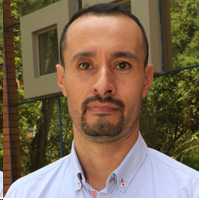
\includegraphics[keepaspectratio]{images/Autores/FAOM.png}}

\section*{\texorpdfstring{Fredy Alejandro Ortiz Meneses
\protect
\includegraphics[width=0.23958in,height=0.28125in]{images/Logos/orcid.png}}{Fredy Alejandro Ortiz Meneses }}\label{fredy-alejandro-ortiz-meneses}
\addcontentsline{toc}{section}{Fredy Alejandro Ortiz Meneses }

\markright{Fredy Alejandro Ortiz Meneses

\includegraphics[width=0.23958in,height=0.28125in]{images/Logos/orcid.png}}

Microbiólogo con énfasis en Alimentos, Especialista en Pedagogía y
Didácticas Específicas, y Magíster en Fitopatología.

\end{tcolorbox}

\begin{tcolorbox}[enhanced jigsaw, titlerule=0mm, arc=.35mm, rightrule=.15mm, bottomrule=.15mm, leftrule=.75mm, colbacktitle=quarto-callout-tip-color!10!white, colframe=quarto-callout-tip-color-frame, coltitle=black, opacityback=0, colback=white, toptitle=1mm, opacitybacktitle=0.6, toprule=.15mm, bottomtitle=1mm, title=\textcolor{quarto-callout-tip-color}{\faLightbulb}\hspace{0.5em}{Tip}, left=2mm, breakable]

\pandocbounded{
\includegraphics[keepaspectratio]{images/Autores/MOPP.jpg}}

\section*{\texorpdfstring{Miguel Oswaldo Pérez Pulido
\protect
\includegraphics[width=0.27083in,height=0.29167in]{images/Logos/orcid.png}}{Miguel Oswaldo Pérez Pulido }}\label{miguel-oswaldo-puxe9rez-pulido}
\addcontentsline{toc}{section}{Miguel Oswaldo Pérez Pulido }

\markright{Miguel Oswaldo Pérez Pulido

\includegraphics[width=0.27083in,height=0.29167in]{images/Logos/orcid.png}}

Director de Analítica Académica. Licenciado en Matemáticas y Magíster en
Estadística. Actualmente se desempeña como Director de Analítica
Académica, adscrito a la Vicerrectoría de Enseñanza. Está vinculado a la
Universidad de Santander (UDES) desde 2011, donde ha sido docente en
programas de pregrado y posgrado de la Facultad de Ciencias Exactas,
Naturales y Agropecuarias. Es investigador Junior reconocido por
Minciencias en la convocatoria 894 de 2021 y miembro del grupo de
investigación CIBAS.

\end{tcolorbox}

\begin{tcolorbox}[enhanced jigsaw, titlerule=0mm, arc=.35mm, rightrule=.15mm, bottomrule=.15mm, leftrule=.75mm, colbacktitle=quarto-callout-tip-color!10!white, colframe=quarto-callout-tip-color-frame, coltitle=black, opacityback=0, colback=white, toptitle=1mm, opacitybacktitle=0.6, toprule=.15mm, bottomtitle=1mm, title=\textcolor{quarto-callout-tip-color}{\faLightbulb}\hspace{0.5em}{Tip}, left=2mm, breakable]

\pandocbounded{
\includegraphics[keepaspectratio]{images/Autores/FJL.jpg}}

\section*{\texorpdfstring{Francisco Javier León
\protect
\includegraphics[width=0.27083in,height=0.29167in]{images/Logos/orcid.png}}{Francisco Javier León }}\label{francisco-javier-leuxf3n}
\addcontentsline{toc}{section}{Francisco Javier León }

\markright{Francisco Javier León

\includegraphics[width=0.27083in,height=0.29167in]{images/Logos/orcid.png}}

Bacteriólogo y laboratorista clínico, con formación avanzada como
Magíster en Estadística Aplicada, Magíster en Ciencias Básicas
Biomédicas y Especialista en Educación con Nuevas Tecnologías. Está
vinculado a la Universidad de Santander (UDES) desde 2007, donde ha sido
docente en la Facultad de Ciencias Exactas, Naturales y Agropecuarias.
Actualmente, se desempeña como Coordinador de Analítica Académica,
adscrito a la Vicerrectoría de Enseñanza. Es investigador Junior
reconocido por Minciencias en la convocatoria 894 de 2021 y miembro del
grupo de investigación CIBAS.

\end{tcolorbox}

\bookmarksetup{startatroot}

\chapter{Agradecimientos}\label{agradecimientos}

\bookmarksetup{startatroot}

\chapter*{Agradecimientos}\label{agradecimientos-1}
\addcontentsline{toc}{chapter}{Agradecimientos}

\markboth{Agradecimientos}{Agradecimientos}

En primer lugar, queremos expresar nuestro más sincero agradecimiento a
todos los estudiantes y profesores del programa de Microbiología que, a
lo largo del tiempo, han compartido con nosotros sus inquietudes y retos
al intentar conectar el análisis estadístico con la microbiología
industrial.

Nuestro agradecimiento se extiende a los colegas académicos,
especialmente a los profesores: Christian Andrey Chacín Zambrano y
Daniel Adyro Martinez; y a los estudiantes graduados que generosamente
compartieron sus experiencias y bases de datos, provenientes de
importantes experimentos académicos. Sus aportes han sido fundamentales
para dar vida a este manual y hacerlo relevante y aplicable a
situaciones reales dentro del contexto de la microbiología industrial.

Asimismo, manifestamos gratitud a Robert Gentleman y Ross Ihaka,
creadores del software R, así como a todos los colaboradores de la
comunidad de R y RStudio®. Gracias a su compromiso y dedicación, estas
herramientas se han mantenido accesibles para la comunidad científica.

A la Universidad de Santander (UDES) y a su Departamento de Desarrollo
Profesoral, por la apertura de la Convocatoria Interna
\textbf{Producción de Material Profesoral (2025)}, gracias a esta
iniciativa, hemos encontrado un espacio de apoyo institucional que
valora la producción material educativo de calidad, gracias a ello, nos
sentimos motivados a seguir desarrollando herramientas que fortalezcan
una enseñanza efectiva en los campos de la Microbiología Industrial y la
Estadística Aplicada.

\bookmarksetup{startatroot}

\chapter{Introducción}\label{introducciuxf3n}

En el ámbito de la microbiología industrial, donde los requerimientos
analíticos varían según el tipo de experimento y los objetivos
investigativos, R y RStudio® ofrecen una flexibilidad sobresaliente. La
comunidad global de usuarios provee soporte constante y recursos
actualizados, mientras que la amplia disponibilidad de paquetes
especializados permite realizar análisis complejos con mayor precisión y
eficiencia (Wickham \& Grolemund, 2017). Esta combinación de potencia
analítica, reproducibilidad y accesibilidad convierte a R en una
herramienta idónea para el análisis de datos experimentales, el diseño
de experimentos y la optimización de procesos biotecnológicos.

El presente libro está estructurado en tres partes principales.

\begin{itemize}
\item
  La Parte I aborda la instalación, configuración y manejo del entorno
  RStudio®, junto con un inventario de librerías esenciales para el
  análisis de datos en microbiología industrial.
\item
  La Parte II desarrolla aplicaciones prácticas de R en el diseño
  experimental, con ejemplos reproducibles de diseños completamente al
  azar, en bloques y con mediciones repetidas en el tiempo.
\item
  La Parte III introduce el uso de inteligencia artificial y simulación
  de datos, explorando cómo los modelos generativos y las herramientas
  computacionales pueden complementar la investigación microbiológica
  moderna.
\end{itemize}

De este modo, el libro ofrece una guía integral que combina fundamentos
teóricos, práctica aplicada y perspectivas innovadoras, contribuyendo a
fortalecer las competencias analíticas de los estudiantes y
profesionales de la microbiología industrial.

\bookmarksetup{startatroot}

\chapter{Parte I: Preparación del Entorno y
Herramientas}\label{parte-i-preparaciuxf3n-del-entorno-y-herramientas}

\section{Introducción al software R y
RStudio}\label{introducciuxf3n-al-software-r-y-rstudio}

\subsection{Instalación y
configuración}\label{instalaciuxf3n-y-configuraciuxf3n}

La instalación de R y RStudio® es un proceso sencillo que puede
completarse en unos pocos pasos; primero, se debe descargar e instalar R
desde el sitio web oficial del Proyecto R
(\url{https://www.r-project.org}); una vez instalado R, se puede
proceder a descargar e instalar RStudio® desde su sitio web
(\url{https://posit.co/download/rstudio-desktop/}) (Figura 1).

\begin{figure}[H]

{\centering \pandocbounded{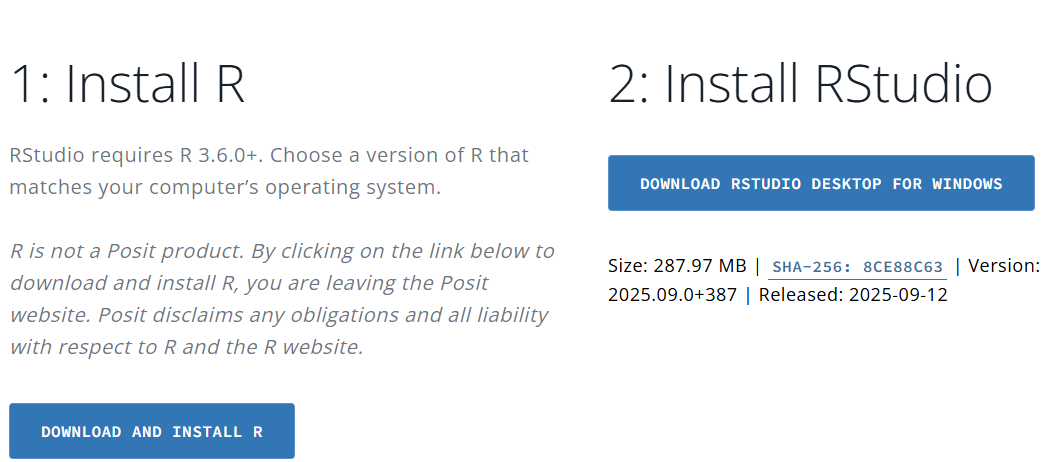
\includegraphics[keepaspectratio]{images/1_Instalacion/Figura 1.png}}

}

\caption{Figura 1.}

\end{figure}%

Ambos programas están disponibles para múltiples sistemas operativos,
incluyendo Windows, macOS y Linux (Figura 2).

\begin{figure}[H]

{\centering \pandocbounded{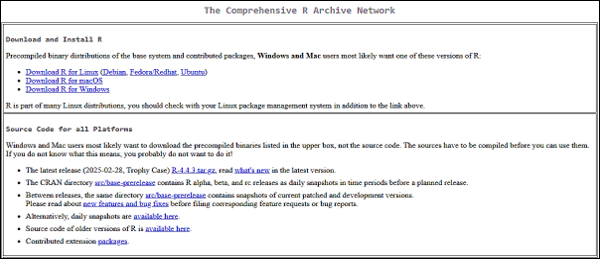
\includegraphics[keepaspectratio]{images/1_Instalacion/Figura 2.png}}

}

\caption{Figura 2.}

\end{figure}%

Del mismo modo se deben descarga de diferentes directorios llamadas CRAN
(Comprehensive R Archive Network o Red integral de archivo R) (Figura
3).

\begin{figure}[H]

{\centering \pandocbounded{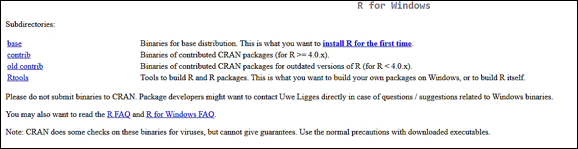
\includegraphics[keepaspectratio]{images/1_Instalacion/Figura 3.png}}

}

\caption{Figura 3.}

\end{figure}%

Finalmente descargar la última versión de R para Windows (Figura 4).

\begin{figure}[H]

{\centering \pandocbounded{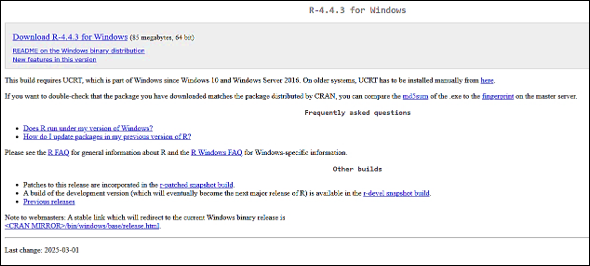
\includegraphics[keepaspectratio]{images/1_Instalacion/Figura 4.png}}

}

\caption{Figura 4.}

\end{figure}%

Una vez instalados R y RStudio®, es importante familiarizarse con la
interfaz de RStudio® (Figura 5); esta interfaz está dividida en varias
secciones, incluyendo: (i) el editor de código o Script, el cual permite
escribir y editar las instrucciones o Scripts; (ii) la consola: se
utiliza para ejecutar comandos interactivos; (iii) el entorno de
trabajo: muestra los objetos y datos cargados en la sesión actual y las
(iv) pestañas de archivos y gráficos: permiten gestionar archivos y
visualizar gráficos generados por R (R Core Team, 2021).

\begin{figure}[H]

{\centering \pandocbounded{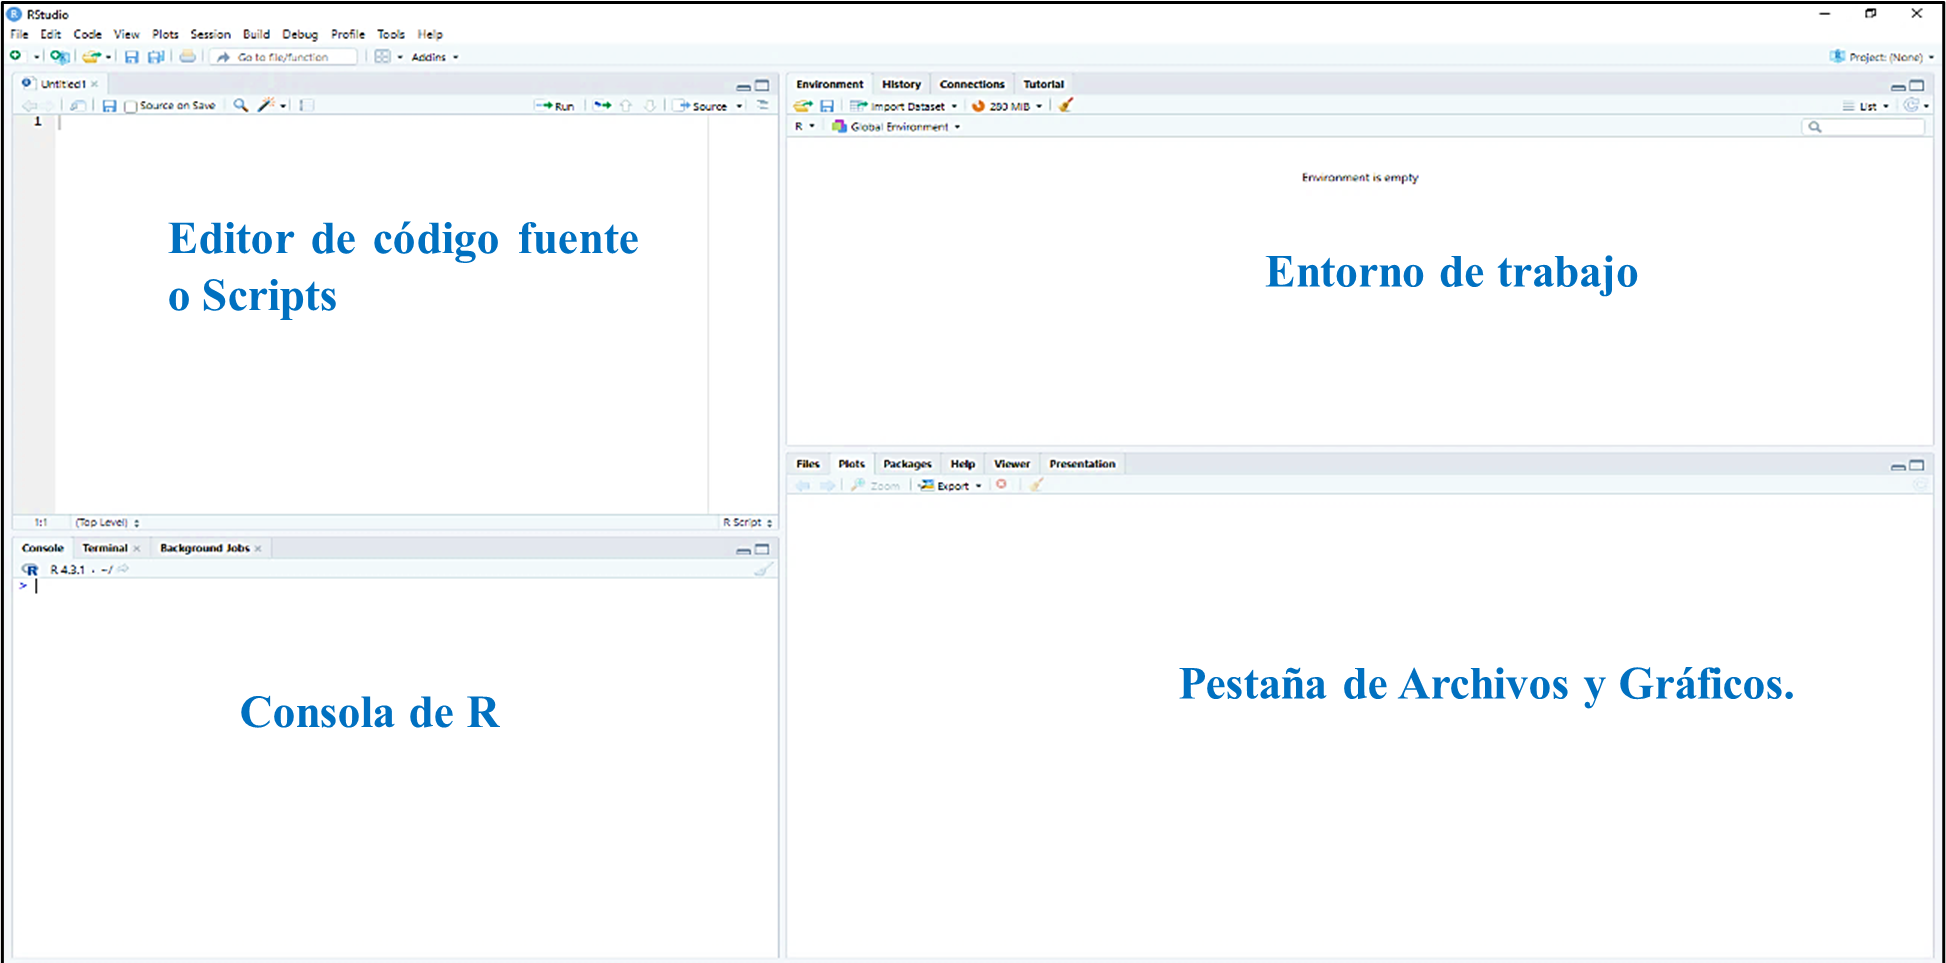
\includegraphics[keepaspectratio]{images/1_Instalacion/Figura 5.png}}

}

\caption{Figura 5}

\end{figure}%

Además de la interfaz básica, RStudio® permite la instalación y gestión
de paquetes adicionales que amplían sus funcionalidades; para instalar
un paquete, se puede utilizar la función install.packages
(``nombre\_del\_paquete'') en la consola de RStudio®; una vez instalado,
el paquete se puede cargar en la sesión actual utilizando la función
library (nombre\_del\_paquete).

\begin{tcolorbox}[enhanced jigsaw, titlerule=0mm, arc=.35mm, rightrule=.15mm, bottomrule=.15mm, leftrule=.75mm, colbacktitle=quarto-callout-important-color!10!white, colframe=quarto-callout-important-color-frame, coltitle=black, opacityback=0, colback=white, toptitle=1mm, opacitybacktitle=0.6, toprule=.15mm, bottomtitle=1mm, title=\textcolor{quarto-callout-important-color}{\faExclamation}\hspace{0.5em}{Importante}, left=2mm, breakable]

Mantener R y RStudio® actualizados es clave para aprovechar las últimas
mejoras, nuevas funcionalidades y correcciones de errores. Ambos
programas notifican automáticamente cuando hay versiones más recientes
disponibles, por lo que se recomienda estar atento a estos avisos y
actualizar oportunamente.

\end{tcolorbox}

Para actualizar R, se debe descargar e instalar la nueva versión desde
el sitio web del Proyecto R; para actualizar RStudio®, se puede utilizar
la opción de actualización en el menú de ayuda de RStudio®; mantener el
software actualizado garantiza un rendimiento óptimo y acceso a las
últimas funcionalidades (R Core Team, 2021) (R Core Team, 2023; RStudio
Team, 2023).

\subsection{Paquetes Esenciales para el análisis de
datos}\label{paquetes-esenciales-para-el-anuxe1lisis-de-datos}

\subsubsection{Inventario de Librerías y Paquetes de R aplicados para el
análisis de datos en Microbiología
Industrial.}\label{inventario-de-libreruxedas-y-paquetes-de-r-aplicados-para-el-anuxe1lisis-de-datos-en-microbiologuxeda-industrial.}

El ecosistema de librerías y paquetes de R constituye una herramienta
fundamental para el análisis de datos en microbiología industrial,
proporcionando soluciones específicas para cada etapa del proceso
investigativo, y en este contexto, las librerías básicas como:

\begin{itemize}
\item
  \href{https://readxl.tidyverse.org/}{\textbf{\emph{readxl}}},
  desarrollada por (Wickham \& Bryan, 2015), facilita la importación de
  datos desde hojas de cálculo Excel®, donde tradicionalmente los
  microbiólogos registran sus resultados experimentales.
\item
  \href{https://cran.r-project.org/web/packages/car/index.html}{\textbf{\emph{car}}}
  (Companion to Applied Regression), creada por (Fox \& Weisberg, 2019),
  ofrece herramientas esenciales para la verificación de supuestos
  estadísticos mediante gráficos QQ-plot, permitiendo evaluar la
  normalidad de los datos antes de aplicar pruebas paramétricas en
  experimentos de optimización de medios de cultivo y comparación de
  cepas microbianas.
\end{itemize}

La revolución en el análisis de datos microbiológicos se materializa
principalmente a través del libreria
\href{https://tidyverse.tidyverse.org/}{\textbf{\emph{tidyverse}}},
desarrollado por (Wickham et~al., 2019), que integra múltiples librerías
bajo una lógica común de programación, Este conjunto incluye los
siguientes paquetes:

\begin{itemize}
\item
  \href{https://ggplot2.tidyverse.org/}{\textbf{ggplot2}} , para
  visualización de datos.
\item
  \href{https://dplyr.tidyverse.org/}{\textbf{dplyr}} , para
  manipulación de datos.
\item
  \href{https://tidyr.tidyverse.org/}{\textbf{tidyr}} , para ordenar
  datos.
\item
  \href{https://readr.tidyverse.org/}{\textbf{readr}} , para importar
  datos.
\item
  \href{https://purrr.tidyverse.org/}{\textbf{purrr}} , para
  programación funcional.
\item
  \href{https://tibble.tidyverse.org/}{\textbf{tibble}} , para tibbles,
  una reinvención moderna de los marcos de datos.
\item
  \href{https://github.com/tidyverse/stringr}{\textbf{stringr}} , para
  cadenas.
\item
  \href{https://github.com/tidyverse/forcats}{\textbf{forcats}} , para
  factores.
\item
  \href{https://github.com/tidyverse/lubridate}{\textbf{lubridate}} ,
  para fecha/hora.
\end{itemize}

Los analísis se enriquecen, considerablemente con librerías
especializadas que abordan necesidades específicas de la investigación
microbiológica industrial, y tal es el caso de:

\begin{itemize}
\item
  \href{https://cran.r-project.org/web/packages/gridExtra/index.html}{\textbf{\emph{gridExtra}}},
  desarrollada por (Auguie, 2017), la cual facilita la organización de
  múltiples gráficos en una sola visualización, permitiendo
  comparaciones efectivas entre diferentes condiciones experimentales.
\item
  \href{https://cran.r-project.org/web/packages/lsr/index.html}{\textbf{\emph{lsr}}}
  (Learning Statistics with R), creada por (Navarro, 2015) proporciona
  funciones accesibles para análisis estadísticos fundamentales como
  pruebas t, ANOVA y cálculos de tamaño del efecto;
\item
  \href{https://www.bibliometrix.org/home/}{\textbf{Bibliometrix}},
  desarrollado por (Aria \& Cuccurullo, 2017) permite realizar análisis
  bibliométrico de publicaciones científicas, identificando tendencias
  emergentes y redes de colaboración que orientan nuevas
  investigaciones.
\end{itemize}

Las aplicaciones especializadas en análisis multivariado y modelado
avanzado complementan este inventario tecnológico, y es donde converge:

\begin{itemize}
\item
  \href{https://cran.r-project.org/web/packages/vegan/index.html}{\textbf{\emph{vegan}}},
  desarrollada por (Oksanen et~al., 2020), la cual proporciona
  proporciona herramientas para análisis de diversidad ecológica
  mediante técnicas como PCA (Análisis de Componentes Principales), NMDS
  (Escalamiento Multidimensional No Métric) permitiendo visualizar
  relaciones complejas entre comunidades microbianas y variables
  ambientales en procesos industriales.
\item
  \href{https://fhernanb.github.io/libro_modelos_mixtos/pac-nlme.html}{\textbf{\emph{nlme}}}
  desarrollado por (Pinheiro et~al., 2025) ofrece capacidades para
  modelar datos longitudinales con estructura jerárquica, típicos de
  estudios de cinética microbiana.
\item
  \href{https://cran.r-project.org/web/packages/agricolae/index.html}{\textbf{\emph{Agricolae}}}
  facilita el diseño experimental(Mendiburu, 2020).
\item
  \href{https://shiny.posit.co/r/getstarted/shiny-basics/lesson1/}{\textbf{\emph{Shiny}}}
  permite desarrollar aplicaciones web interactivas para visualización
  dinámica de resultados, mejorando la colaboración y transparencia en
  la investigación microbiológica industrial(Chang et~al., 2021).
\end{itemize}

\subsubsection{Uso de R en Microbiología
Industrial}\label{uso-de-r-en-microbiologuxeda-industrial}

El uso de R como herramienta de análisis estadístico en la microbiología
industrial ha experimentado un crecimiento exponencial en la última
década, según (Mohammadi et~al., 2019) R proporciona una plataforma
versátil que permite analizar datos complejos derivados de experimentos
microbiológicos, facilitando la identificación de patrones de
crecimiento microbiano, optimización de condiciones de cultivo y
evaluación de la producción de metabolitos secundarios, lo que resulta
crucial para el desarrollo y mejora de procesos biotecnológicos en
entornos industriales.

(McMurdie \& Holmes, 2013) desarrollaron el paquete \emph{phyloseq}, el
cual ha transformado el análisis de datos de secuenciación en estudios
de comunidades microbianas, permitiendo la integración de información
taxonómica, filogenética y de abundancia en un solo entorno analítico;
este avance ha sido fundamental para comprender la dinámica de
\textbf{poblaciones microbianas} en procesos industriales como: el
tratamiento de aguas residuales, la producción de biocombustibles y la
fermentación alimentaria.

Por otra parte, el paquete microbiome, descrito por (Lahti \& Shetty,
2017), proporciona herramientas especializadas para el análisis de
\textbf{datos metagenómicos}, facilitando la caracterización de
comunidades microbianas y sus funciones metabólicas en entornos
industriales, lo que resulta esencial para la optimización de
bioprocesos y el control de calidad en la industria alimentaria.

El \textbf{diseño experimental} en microbiología industrial se ha
beneficiado significativamente de la aplicabilidad de R, permitiendo
planificar y analizar experimentos de manera más rigurosa y eficiente,
el paquete \emph{agricolae}, desarrollado por de Mendiburu (2021) (Zhou
et~al., 2012) es utilizado para la implementación de diseños
experimentales complejos como: bloques aleatorizados y diseños
factoriales entre otros, al tiempo que frecuentemente son utilizados en
estudios de optimización de medios de cultivo, condiciones de
fermentación y producción de enzimas microbianas.

Complementariamente, (Ritz \& Streibig, 2005) presentaron el paquete
\emph{drc} (Dose-Response Curves), que ha facilitado el análisis de
\textbf{Curvas dosis-respuesta} en estudios de inhibición microbiana,
pruebas de susceptibilidad a antimicrobianos y evaluación de compuestos
bioactivos producidos por microorganismos, proporcionando herramientas
estadísticas robustas para cuantificar y modelar respuestas biológicas a
diferentes tratamientos, lo cual es fundamental en el desarrollo de
nuevos productos biotecnológicos.

El paquete \emph{ggplot2} desarrollado por (Wickham, 2016), el cual ha
permitido la creación de gráficos altamente informativos que facilitan
la interpretación de resultados experimentales; en particular, la
representación gráfica de cinéticas de crecimiento microbiano,
producción de metabolitos y análisis multivariantes se ha vuelto más
accesible e intuitiva para investigadores en el campo; de manera similar
el paquete \emph{ggtree}, creado por (Yu et~al., 2017), ha revolucionado
la visualización de datos filogenéticos en estudios de diversidad
microbiana industrial, permitiendo representar relaciones evolutivas
entre microorganismos de interés biotecnológico y correlacionarlas con
características fenotípicas relevantes para procesos industriales, lo
que facilita la selección de cepas microbianas con potencial
biotecnológico.

\begin{tcolorbox}[enhanced jigsaw, titlerule=0mm, arc=.35mm, rightrule=.15mm, bottomrule=.15mm, leftrule=.75mm, colbacktitle=quarto-callout-caution-color!10!white, colframe=quarto-callout-caution-color-frame, coltitle=black, opacityback=0, colback=white, toptitle=1mm, opacitybacktitle=0.6, toprule=.15mm, bottomtitle=1mm, title=\textcolor{quarto-callout-caution-color}{\faFire}\hspace{0.5em}{Expandir para aprender son el analis de datos ómicos}, left=2mm, breakable]

El análisis de datos ómicos en microbiología industrial se ha visto
significativamente potenciado gracias al aporte de (Love et~al., 2014)
quienes introdujeron \emph{DESeq2}, un paquete que ha transformado el
análisis de datos de RNA-seq en estudios transcriptómicos de
microorganismos industriales, permitiendo identificar genes
diferencialmente expresados bajo diversas condiciones de cultivo o
modificaciones genéticas; lo que contribuye a la mejora de cepas
microbianas industriales y a optimizar rutas metabólicas de interés
comercial; paralelamente (Rohart et~al., 2017) desarrollaron el paquete
mixOmics, el cual facilita la integración de múltiples conjuntos de
datos ómicos, como:

\begin{enumerate}
\def\labelenumi{(\roman{enumi})}
\tightlist
\item
  transcriptómica,
\item
  proteómica y
\item
  metabolómica,
\end{enumerate}

proporcionando una visión holística de los sistemas microbianos en
contextos industriales, lo que permite desentrañar complejas redes
regulatorias y metabólicas que subyacen a procesos biotecnológicos
importantes como de compuestos bioactivos.

\end{tcolorbox}

\section{Análisis Bibliométrico para el Diseño de Experimentos y la
Microbiología
Industrial}\label{anuxe1lisis-bibliomuxe9trico-para-el-diseuxf1o-de-experimentos-y-la-microbiologuxeda-industrial}

El paquete
\href{https://www.bibliometrix.org/home/}{\textbf{Bibliometrix}},
desarrollado en R, constituye una herramienta clave para el análisis
bibliométrico en distintas áreas del conocimiento, entre ellas la
\href{https://bucaramanga.udes.edu.co/estudia/pregrados/microbiologia-industrial}{\textbf{microbiología
industrial}} y el \textbf{diseño experimental}. Su enfoque de código
abierto permite recopilar, analizar y visualizar información científica
de manera integral, ofreciendo una visión clara sobre las principales
tendencias y la evolución de la investigación en cada campo (Aria \&
Cuccurullo, 2017).

En la \textbf{microbiología industrial},
\href{https://www.bibliometrix.org/home/}{\textbf{Bibliometrix}} se ha
convertido en un apoyo fundamental para reconocer \textbf{líneas
emergentes de investigación}, \textbf{colaboraciones internacionales} y
\textbf{autores influyentes} que marcan el desarrollo del área (Aria \&
Cuccurullo, 2017). A través de su interfaz visual
\href{https://www.bibliometrix.org/home/index.php/layout/biblioshiny}{\textbf{Biblioshiny}},
los análisis complejos se vuelven accesibles incluso para quienes no
tienen experiencia en programación. Esta accesibilidad favorece la
creación de \textbf{mapas de conocimiento}, \textbf{redes de
colaboración} y \textbf{agrupamientos temáticos} que ayudan a
identificar oportunidades de trabajo conjunto, vacíos en la literatura o
la evolución de determinadas técnicas experimentales.

El uso de Bibliometrix y Biblioshiny permite una comprensión argumentada
del panorama científico, fomentando decisiones de investigación basadas
en evidencia y fortaleciendo la planificación de proyectos dentro de la
microbiología industrial.

\subsection{Procedimiento para el Análisis Bibliométrico con
Bibliometrix a partir de una Base de Datos
Scopus}\label{procedimiento-para-el-anuxe1lisis-bibliomuxe9trico-con-bibliometrix-a-partir-de-una-base-de-datos-scopus}

Como ejemplo de análisis bibliometrico se emplearán los datos de trabajo
de grado titulado (sin publicar) ``Evaluación del crecimiento de
\emph{Cordyceps militaris} en diferentes sustratos vegetales''(Chala,
2025).

\subsection{Palabras clave, operadores Booleanos y búsqueda en bases de
datos}\label{palabras-clave-operadores-booleanos-y-buxfasqueda-en-bases-de-datos}

El primer paso consiste en generar cinco palabras claves relacionadas
con el tema de estudio, como son:

\begin{enumerate}
\def\labelenumi{\arabic{enumi}.}
\item
  \emph{Cultivation}: proceso de cultivar \emph{Cordyceps militaris} en
  condiciones controladas paraestudiar su crecimiento y desarrollo.
\item
  \emph{Mycelial grow}th: crecimiento del micelio, la parte vegetativa
  del hongo, que escrucial para evaluar su desarrollo.
\item
  \emph{Substrate optimization}: mejora de los sustratos utilizados para
  el cultivo del hongo, conel fin de maximizar su crecimiento y
  producción de compuestos bioactivos.
\item
  \emph{Bioactive compound}s: compuestos producidos por Cordyceps
  militaris, como la cordicepina, quetienen propiedades medicinales y
  son un indicador de la calidad del crecimiento.
\item
  \emph{Fermentation condition}s: condiciones de fermentación, como la
  temperatura, pH y nutrientes, que afectan el crecimiento y la
  producción de metabolitos del hongo.
\end{enumerate}

El segundo paso es generar diez (10) ecuaciones de búsqueda ingresando a
una de las siguientes base de revistas indexadas compatibles con
Bibliometrix, como son: Web of Science
(\href{http://www.webofscience.com}{www.webofscience.com}), Scopus
(\href{http://www.scopus.com}{www.scopus.com}); OpenAlex
(\href{http://www.openalex.org}{www.openalex.org}); Dimensions
(\href{http://www.dimensions.ai}{www.dimensions.ai}); The Lens
(\href{http://www.lens.org}{www.lens.org}); PubMed
(\url{https://pubmed.ncbi.nlm.nih.gov/}) y Cochrane Library
(\href{http://www.cochranelibrary.com/}{www.cochranelibrary.com/}),
desde donde se utilizaran operadores booleanos relacionados con el tema,
es importante que cada una de las palabras clave estén encerradas entre
comillas '' '' ; al tiempo que se utilicen los conectores: AND y/o OR y
NOT para refinar la búsqueda, como se muestran a continuación:

\begin{itemize}
\item
  ``\emph{Cordyceps militaris}'' AND ``growth evaluation''
\item
  ``\emph{Cordyceps militaris}'' AND (``substrate optimization'' OR
  ``culture medium'') AND ``growth''
\item
  ``Cordyceps militaris'' AND ``cordycepin'' AND ``growth''
\item
  ``\emph{Cordyceps militaris}'' AND ``temperature'' AND ``mycelial
  growth''
\item
  ``\emph{Cordyceps militaris}'' AND ``fermentation'' AND (``solid-state
  fermentation'')
\item
  ``\emph{Cordyceps militaris}'' AND (``natural growth'' OR ``artificial
  cultivation'') AND (``yield'' OR ``biomass production'')
\item
  ``\emph{Cordyceps militaris}'' AND (``metabolite profiling'' OR
  ``secondary metabolites'') AND ``growth conditions''
\item
  ``\emph{Cordyceps militaris}'' AND (``carbon source'' OR ``nitrogen
  source'') AND ``mycelial biomass''
\item
  ``\emph{Cordyceps militaris}'' AND (``rice medium'' OR ``wheat
  medium'' OR ``synthetic medium'') AND ``growth performance''
\item
  ``\emph{Cordyceps militaris}'' AND ``commercial production'' AND
  (``growth enhancement'' OR ``yield improvement''
\end{itemize}

En la Tabla 1, se aprecian el número de publicaciones científicas
relacionadas con algunas de las ecuanciones de búsqueda, lo que
permitirá la elección del resultado más promisorio, para seguidamente
proceder con el proceso de descarga de los metadatos en formato .csv.

\begin{longtable}[]{@{}
  >{\raggedright\arraybackslash}p{(\linewidth - 2\tabcolsep) * \real{0.7361}}
  >{\raggedright\arraybackslash}p{(\linewidth - 2\tabcolsep) * \real{0.2639}}@{}}
\caption{Tabla 1. Salida de resultados para cada uno de los operadores
booleanos, introducidos dentro de la plataforma de Scopus®, y que están
con el tema de investigación de Cordyceps militaris.}\tabularnewline
\toprule\noalign{}
\begin{minipage}[b]{\linewidth}\raggedright
Ecuación de búsqueda
\end{minipage} & \begin{minipage}[b]{\linewidth}\raggedright
Documentos encontrados
\end{minipage} \\
\midrule\noalign{}
\endfirsthead
\toprule\noalign{}
\begin{minipage}[b]{\linewidth}\raggedright
Ecuación de búsqueda
\end{minipage} & \begin{minipage}[b]{\linewidth}\raggedright
Documentos encontrados
\end{minipage} \\
\midrule\noalign{}
\endhead
\bottomrule\noalign{}
\endlastfoot
``Cordyceps militaris'' AND (``metabolite'' OR ``growth conditions'' &
225 \\
``Cordyceps militaris'' AND (``cordycepin'') AND ``growth'' & 191 \\
``Cordyceps militaris'' AND ``medium'' AND ``growth'' & 99 \\
``Cordyceps militaris'' AND (``substrate optimization'' OR ``culture
medium'') AND ``growth'' & 40 \\
\end{longtable}

\subsection{Analísis con
bibliometrix}\label{analuxedsis-con-bibliometrix}

Para iniciar el análisis bibliométrico, se procede a ingresar al
programa RStudio®, al tiempo que se realiza la instalación de los
paquetes: \emph{bibliometrix} y \emph{bibliometrixData}, desde la
pestaña de Archivos y Gráficos en la sección de Packages (Figura 8).

\begin{figure}[H]

{\centering \pandocbounded{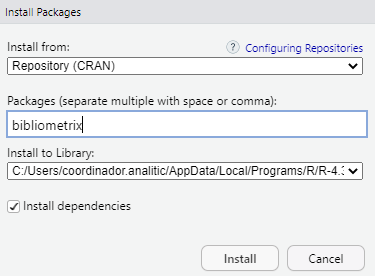
\includegraphics[keepaspectratio]{images/2_Bibliometrix/Bibliometrix1.PNG}}

}

\caption{Figura 8.}

\end{figure}%

Posteriormente, desde la Consola de RStudio se digitan y ejecutan los
comandos:

\begin{quote}
library(bibliometrix) biblioshiny()
\end{quote}

Tambien se puede habilitar manualmente en la pestaña de Archivos y
Graficos de la interfaz de RStudio, pestaña de Packages (figura9)
seleccionado las librerias a usar.

\begin{figure}[H]

{\centering \pandocbounded{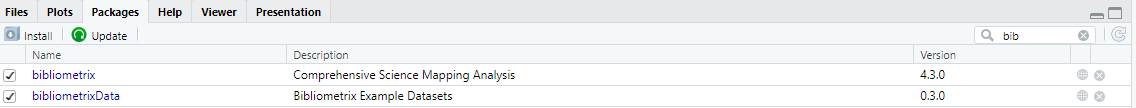
\includegraphics[keepaspectratio]{images/2_Bibliometrix/Bibliometrix2.PNG}}

}

\caption{Figura 9.}

\end{figure}%

Se abrirá el servidor de Bibliometrix (Figura 9) en el navegador web
(Chrome, Mozilla, Edge, entre otros). Es importante aclarar que la
interfaz de Bibliometrix únicamente pude ser ejecutada desde RStudio®.

\begin{figure}[H]

{\centering \pandocbounded{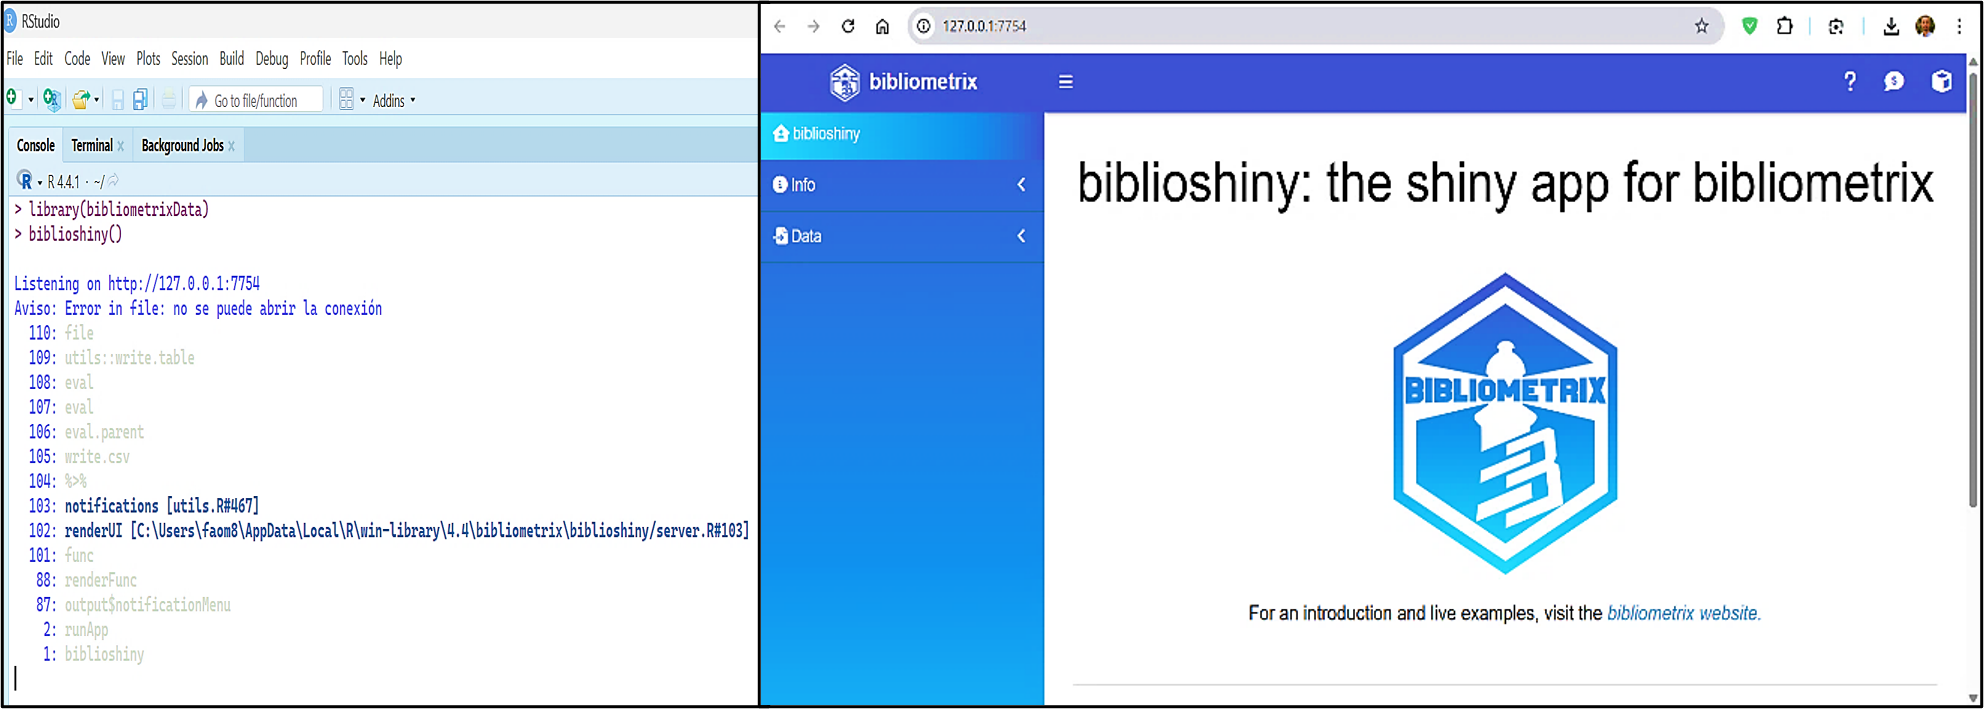
\includegraphics[keepaspectratio]{images/2_Bibliometrix/Figura_9.png}}

}

\caption{Figura 9.}

\end{figure}%

En la parte izquierda se despliega el menú de biblioshiny, y se procede
con la importación en ``\emph{Import or Load}'' se carga el archivo CSV
(Aria \& Cuccurullo, 2017), al tiempo que se seleccionan las casillas:
\emph{Import raw file(s}), la procedencia de la base de datos consultada
(\emph{Scopus,} en nuestro caso) , junto la opción: \emph{Surname and
Initials}, y finalmente damos click en el botón de \emph{Start} ~(Figura
10).

\begin{figure}[H]

{\centering \pandocbounded{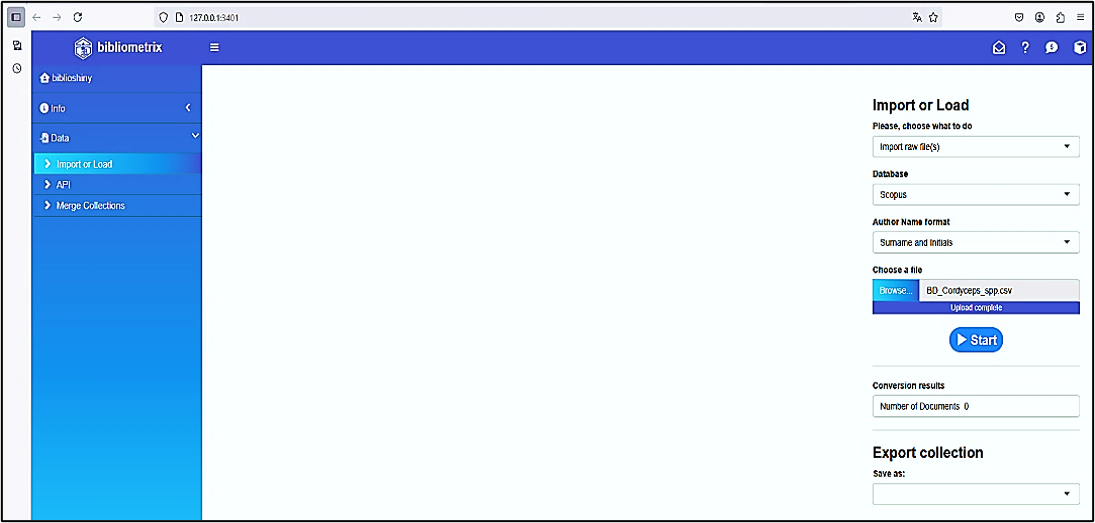
\includegraphics[keepaspectratio]{images/2_Bibliometrix/Figura_10.png}}

}

\caption{Figura 10.}

\end{figure}%

Después se despliega una nueva ventana que muestra el estado de los
componentes de los metadatos importados desde el archivo CSV (Figura
11), allí se muestra una tabla que resume la completitud de los
metadatos (para nuestro ejemplo: 191 documentos de Scopus),.

\begin{figure}[H]

{\centering \pandocbounded{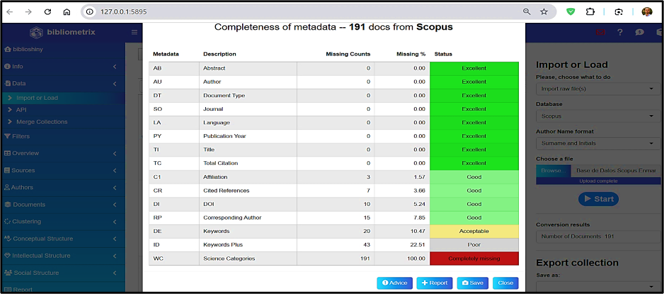
\includegraphics[keepaspectratio]{images/2_Bibliometrix/Figura_11.png}}

}

\caption{Figura 11.}

\end{figure}%

Así mismo Bibliometrix evalúa cada uno de los diferentes campos de
metadatos (Abstract, afiliación, autor, tipo de documento, etc.)
utilizando \emph{junto a} diferentes criterios de clasificación como
son: ``Excelente'', ``Bueno'', ``Aceptable'' ``Pobre'' y ``Completamente
perdido'' (Figura 11), y que al ser cerrado ``Close'' muestra una tabla
dinámica con todos los datos importados incluyendo el DOI, desde el cual
se puede acceder y leer directamente el articulo científico (Figura 12).

\begin{figure}[H]

{\centering \pandocbounded{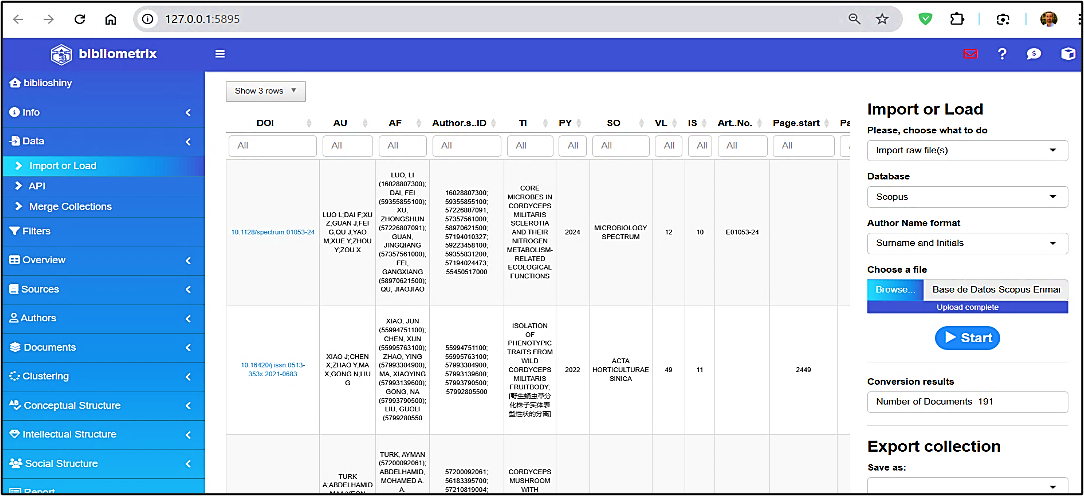
\includegraphics[keepaspectratio]{images/2_Bibliometrix/Figura_12.png}}

}

\caption{Figura 12}

\end{figure}%

\textbf{Bibliometrix} (a través de su interfaz \textbf{Biblioshiny})
está estructurado en \textbf{8 módulos principales} o menús, y dentro de
cada uno hay \textbf{submódulos o indicadores específicos}.

\begin{longtable}[]{@{}
  >{\raggedleft\arraybackslash}p{(\linewidth - 6\tabcolsep) * \real{0.0725}}
  >{\raggedright\arraybackslash}p{(\linewidth - 6\tabcolsep) * \real{0.1884}}
  >{\raggedright\arraybackslash}p{(\linewidth - 6\tabcolsep) * \real{0.3478}}
  >{\raggedright\arraybackslash}p{(\linewidth - 6\tabcolsep) * \real{0.3913}}@{}}
\caption{Módulos principales de Bibliometrix /
Biblioshiny}\label{tbl-bibliometrix}\tabularnewline
\toprule\noalign{}
\begin{minipage}[b]{\linewidth}\raggedleft
Nº
\end{minipage} & \begin{minipage}[b]{\linewidth}\raggedright
Módulo
\end{minipage} & \begin{minipage}[b]{\linewidth}\raggedright
Función general
\end{minipage} & \begin{minipage}[b]{\linewidth}\raggedright
Submódulos / indicadores
\end{minipage} \\
\midrule\noalign{}
\endfirsthead
\toprule\noalign{}
\begin{minipage}[b]{\linewidth}\raggedleft
Nº
\end{minipage} & \begin{minipage}[b]{\linewidth}\raggedright
Módulo
\end{minipage} & \begin{minipage}[b]{\linewidth}\raggedright
Función general
\end{minipage} & \begin{minipage}[b]{\linewidth}\raggedright
Submódulos / indicadores
\end{minipage} \\
\midrule\noalign{}
\endhead
\bottomrule\noalign{}
\endlastfoot
1 & \textbf{Data} & Importar/cargar bases bibliográficas (Scopus, WoS,
PubMed, etc.). & Import or Load; Merge Datasets \\
2 & \textbf{Filters} & Filtrar el corpus por año, tipo de documento,
autores, países, palabras clave. & Time Span; Authors; Countries \\
3 & \textbf{Overview} & Panorama general con indicadores descriptivos. &
Main Information; Annual Scientific Production; Average Citations per
Year; Three-Field Plot \\
4 & \textbf{Sources} & Análisis de revistas/fuentes. & Most Relevant
Sources; Bradford's Law \\
5 & \textbf{Authors} & Productividad, impacto y colaboración de autores.
& Authors' Production Over Time; Most Cited Authors; Collaboration
Network \\
6 & \textbf{Documents} & Documentos más citados y patrones de citación.
& Most Cited Documents; Reference Spectroscopy \\
7 & \textbf{Clustering (Conceptual Structure)} & Estructura
temática/conceptual del campo. & Co-occurrence Network; Thematic Map;
Factorial Analysis \\
8 & \textbf{Social Structure} & Redes de colaboración entre autores,
instituciones y países. & Collaboration Network; Country Scientific
Production; Collaboration World Map \\
\end{longtable}

En el modulo \textbf{\emph{Overview}} se despliega el indicador
\textbf{\emph{Main information}} (Traducido: Información Principal),
donde se muestran los valores de los metadatos descargas, para este
ejemplo: El análisis bibliométrico abarca el periodo de 1951 a 2025 con
un total de 135 fuentes y 191 documentos, la tasa de crecimiento anual
es de 0,94\%, se identificaron 903 autores, sin registros un solo autor;
la coautoría internacional alcanza un valor de 15,18\% y el promedio de
coautores por documento es de 6,19. Se encontraron 543 palabras clave de
autor y 7474 referencias, la edad promedio de los documentos es de 7,34
años y la cantidad media de citas por documento es de 25,69 (Figura 13).

\begin{figure}[H]

{\centering \pandocbounded{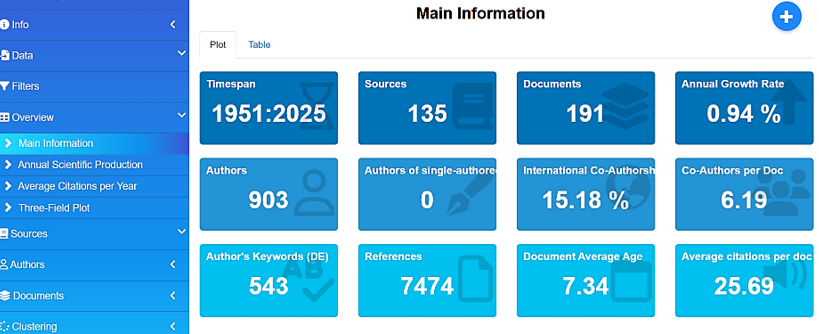
\includegraphics[keepaspectratio]{images/2_Bibliometrix/Figura_13.png}}

}

\caption{Figura 13}

\end{figure}%

En la sección \textbf{\emph{Annual Scientific Production}} (traducido:
Producción Científica Anual) y se muestra que: la evolución de la
cantidad de artículos científicos relacionados con \emph{Cordyceps
militaris} publicados por año, van desde 1951 hasta aproximadamente el
año 2000, la producción científica es muy baja, con solo unos pocos
artículos publicados anualmente; a partir del 2000, se observa un ligero
aumento en la cantidad de publicaciones, pero es a partir de 2010 cuando
el crecimiento se acelera considerablemente, reflejando una tendencia
ascendente más marcada. Entre 2015 y 2024, la producción científica
alcanza sus niveles más altos, con un notable incremento en la cantidad
de artículos publicados cada año. Sin embargo, en 2025 se observa una
caída significativa, lo que podría deberse a datos incompletos, retrasos
en las publicaciones o factores externos como cambios en políticas de
financiamiento o publicación (Figura 14).

\pandocbounded{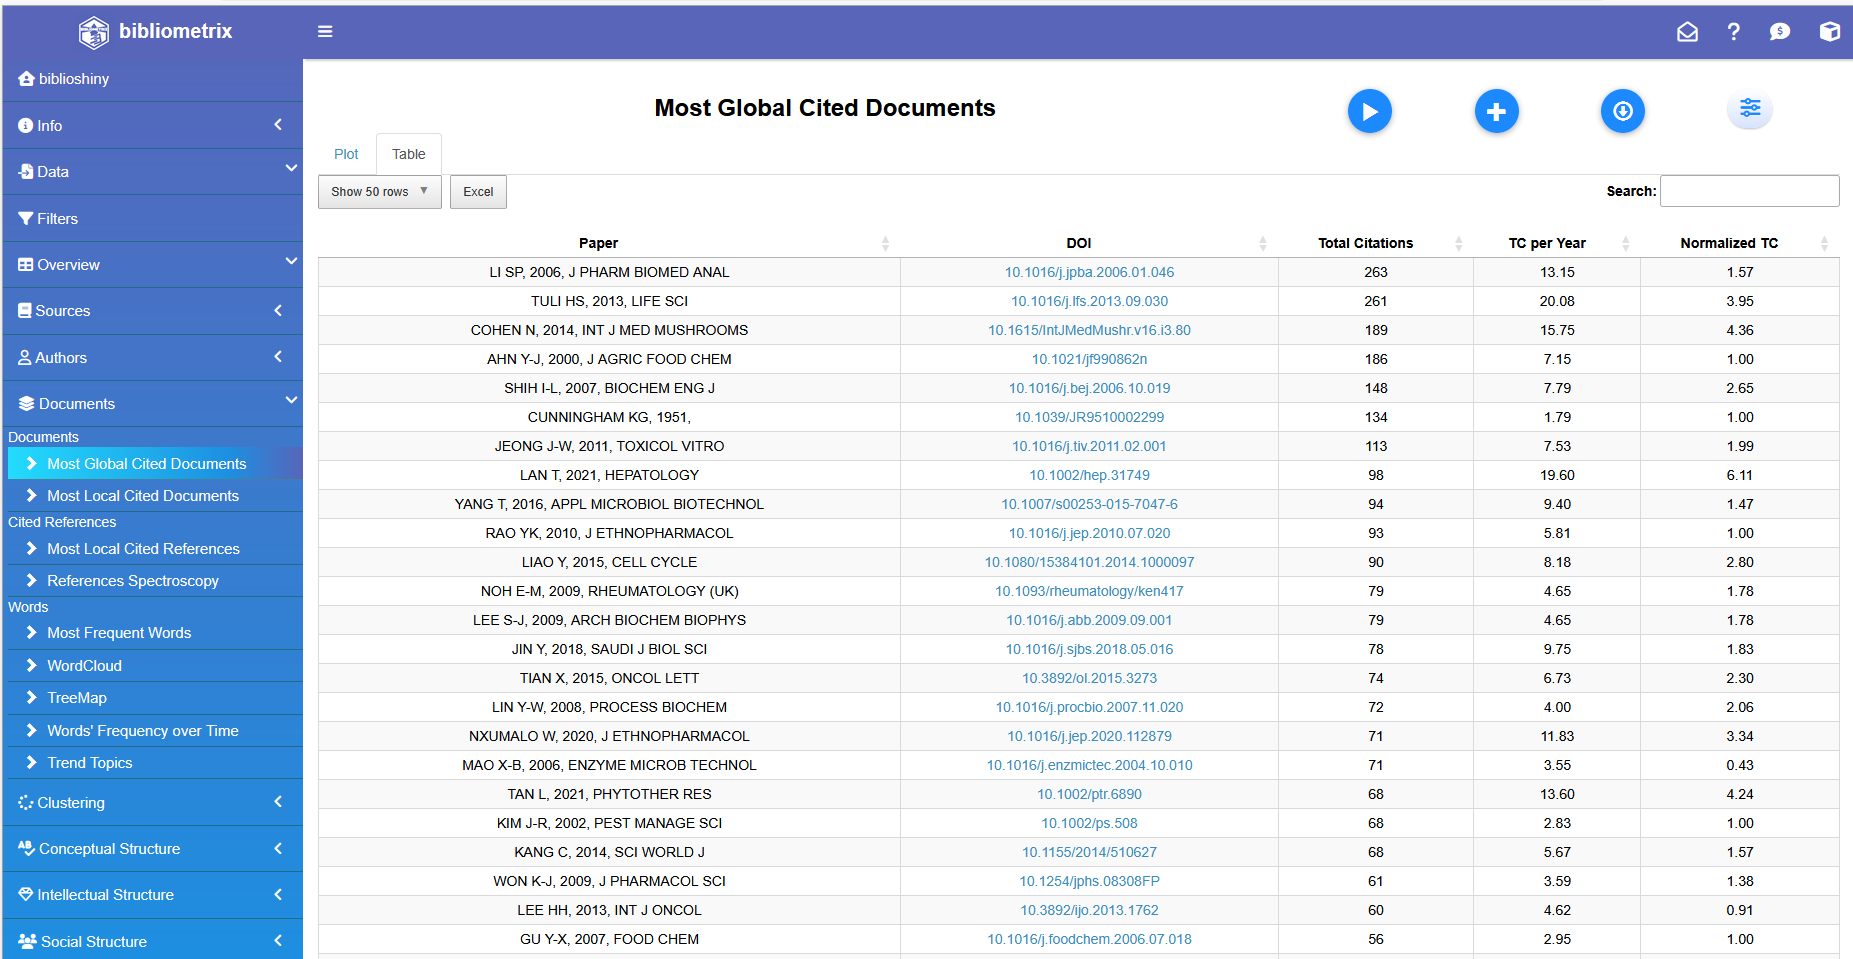
\includegraphics[keepaspectratio]{images/2_Bibliometrix/Bibliometrix12.PNG}}

Para la sección \textbf{\emph{Average Citations Per Ye}ar} (Traducido:
Citas Promedio por año) se muestra la evolución del número promedio de
citas recibidas por los artículos a lo largo del tiempo. Para nuestro
ejemplo didáctico en la temática de Cordyceps militaris, específicamente
en 1951 y 1961, se observan valores relativamente altos, pero con pocos
artículos publicados en esos períodos. Posteriormente, durante varias
décadas, el número promedio de citas se mantiene bajo y estable. A
partir del año 2000 aproximadamente , hay un incremento notable en la
cantidad de citas por artículo, alcanzando picos significativos en el
2006 y 2008 (Figura 15).

\pandocbounded{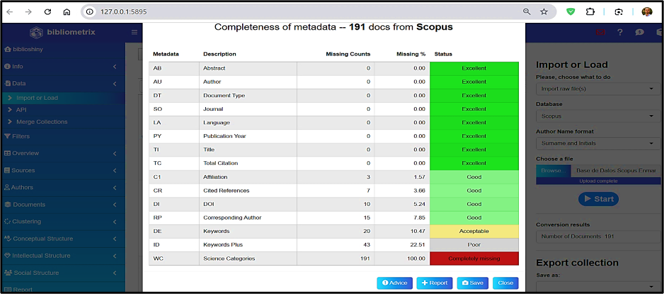
\includegraphics[keepaspectratio]{images/2_Bibliometrix/Figura_11.png}}

No corresponde

Para el menú de \emph{Overview} específicamente en la sección
\textbf{\emph{Three-Field Plot}} (Traducido: Trazo de tres campos) se
proporciona una visión general de la colaboración en investigación y los
temas principales dentro de un cuerpo específico de literatura.
\emph{AU\_CO (Países)}: Muestra la participación de China, Tailandia,
Reino Unido, Singapur, estados Unidos , entre otros; en los artículos
analizados. China lidera la investigación del tema, sugiriendo una
fuerte presencia investigadora en el área del estudio; \emph{AU
(Autores)}: destaca a: Li X, Li Y, Vongsangnak W y Zhang J, como los
autores más productivos, al tiempo que muestra posibles colaboraciones o
equipos de investigación.; \emph{DE (Descriptores)}: Los términos que se
asocian el estudio del hongo \emph{Cordyceps militari}s, la
biotecnología del hongo, compuestos bioactivos y análisis
transcriptómico. Este gráfico reafirma el liderazgo asiático en esta
línea de investigación, así como la concentración temática en los
compuestos bioactivos de Cordyceps militaris y su aplicación en salud y
biotecnología (Figura 16). Importante destacar que Bibliometrix permite
cambiar los parametros de análisis y el número de ítems.

\begin{figure}[H]

{\centering \pandocbounded{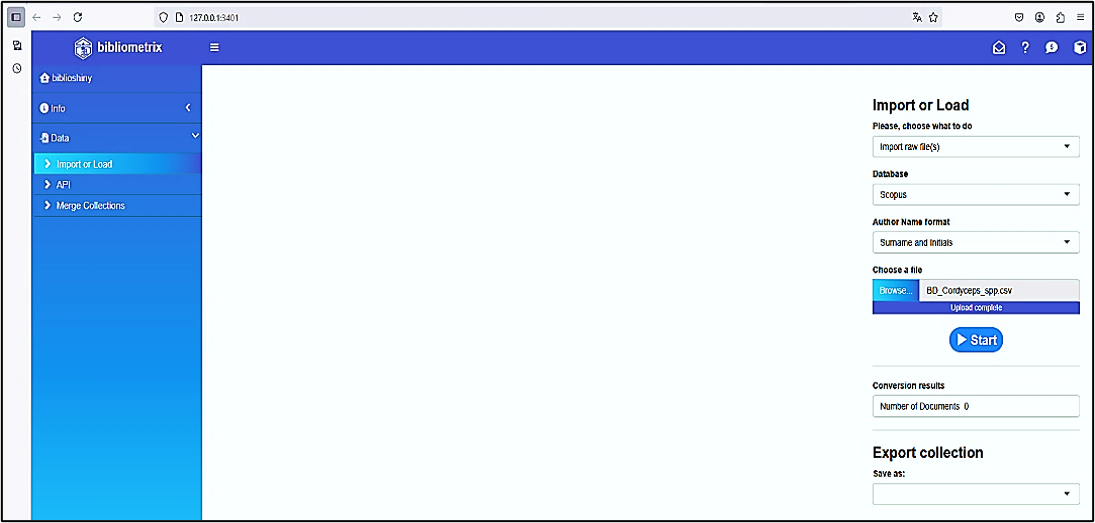
\includegraphics[keepaspectratio]{images/2_Bibliometrix/Figura_10.png}}

}

\caption{Figura 14.}

\end{figure}%

Para el menú de \emph{Sources} en la sección \textbf{\emph{Most Relevant
Sources}} (Traducido: Fuentes más Relevantes) la producción científica
procedente de Scopus está lideradas por: International Journal of
Medicinal Mushrooms con 15 artículos publicados, seguido de Mycosystema
con 8, le sigue: Applied Microbiology and Biotechnology con 5. Dichas
revistas destacan por su enfoque en microbiología, biotecnología y
farmacología, áreas clave dentro del estudio abordado. La distribución
sugiere que la investigación en este campo se encuentra bien
representada en revistas especializadas,las demás revistas como:
Biology, Bioresource Technolgy, y Nutrients, que cuentan con 3 artículos
cada una (Figura 17).

\pandocbounded{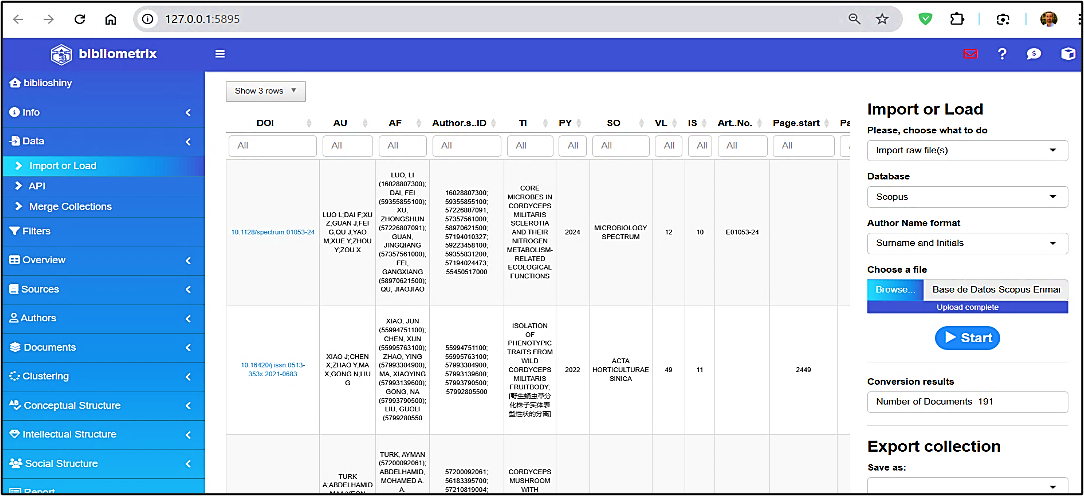
\includegraphics[keepaspectratio]{images/2_Bibliometrix/Figura_12.png}}

No corresponde

En la sección de \textbf{Bradford's Law} (Traducido: La Ley de Bradford)
y continuando con nuestro ejemplo didáctico de \emph{Cordyceps
mil}itaris ,se observa que: ``International Journal of Medicinal
Mushrooms'', junto con ``Mycosystema'' y ``Applied Microbiology and
Biotechnology'', conforman el núcleo de fuentes indexadas ~más
relevantes, aportando el mayor número de publicaciones, estas tres
revistas están dentro del área sombreada, lo que confirma su papel
central en la diseminación del conocimiento sobre \emph{C. militari}s y
compuestos bioactivoss. A medida que se avanza hacia la derecha del
gráfico, el número de artículos por revista disminuye, lo que representa
publicaciones de interés más disperso (Figura 18).

Para el menú de \emph{Authors} específicamente en:
\textbf{\emph{Authors' Production over Time}} (traducido: La producción
de los autores a lo largo del tiempo) se muestra que investigadores:
~Wang Y., Li X., y Li Y., han mantenido una producción constante en los
últimos años, con picos significativos en 2020 y 2022. La visualización
indica que hay una concentración de publicaciones en los últimos cinco
años, lo que sugiere un crecimiento en la investigación dentro de este
campo. Otros autores, como Vongsangnak W. y Zhang J., han contribuido de
manera más esporádica, pero siguen participando activamente en la
investigación del hongo \emph{Cordyceps militaris} (Figura 19).

Para el menú de \emph{Authors} específicamente en:
\textbf{\emph{Countries' Scientific Production}} (traducido: Producción
científica de los países), el mapa muestra la distribución geográfica de
la producción científica. China es el país con mayor producción
científica (azul oscuro); otros países con destacada producción
científica entre los que se incluyen: Estados Unidos, Corea del Sur,
Tailandia, Japón, India y varios países europeos y asiáticos (azul
celeste). Algunos países no presentan producción registrada y aparecen
coloreados en gris. En la tabla se observa que China lidera con 702
publicaciones, seguida por Corea del Sur con 212, Tailandia con 83,
Japón con 50 e India con 39. Otros países con menor producción incluyen
Estados Unidos con 9, Reino Unido con 8, Alemania con 7, Italia con 6 y
Colombia con 5 (Figura 20).

Para el menú de \emph{Document} específicamente en: \textbf{\emph{Most
Frequent Words}} (traducido: Palabras más frecuentes), la visualización
muestra las palabras de uso frecuente con el tema de investigación de
Cordyceps militaris son: Cordyceps con 196 apariciones y Cordycepin con
187. Otras palabras destacadas incluyen article con 109, Cordyceps
militaris con 108, nonhuman con 92, metabolism con 79, deoxyadenosines
con 77, controlled study con 76, deoxyadenosine derivative con 65 y
adenosine con 64 (figura 21).

Para el menú de \emph{Document} específicamente en:
\textbf{\emph{Reference Spectroscopy}} (traducido: Espectroscopia de
referencias), la visualización muestra la evolución de las referencias
citadas en espectroscopia a lo largo del tiempo; antes de 1990, el
número de referencias citadas se mantuvo prácticamente nulo y a partir
de 1995, se observa una pendiente creciente sostenida, que se acelera
alrededor del año 2005, alcanzando su punto máximo entre 2015 y 2020 con
más de 400 referencias citadas por año, después de 2018, se evidencia
una disminución en el número de referencias citadas. También se puede
observar una caída abrupta después del 2020 que puede explicarse por
efectos de rezago en la citación, ya que las publicaciones recientes aún
no han tenido suficiente tiempo para acumular cita (Figura 22).

Para el menú de \emph{Conceptual Structure} concretamente en:
\textbf{\emph{Co-occurrence Network}} (traducido: Red de Coocurrencias),
la red se encuentra claramente dividida en dos comunidades principales,
identificadas por los colores rojo y azul. La comunidad roja, dominada
por términos como cordycepin, Cordyceps militaris, metabolism y article,
se orienta al estudio bioquímico y farmacológico del compuesto, mientras
que la comunidad azul está asociada a modelos experimentales, destacando
términos como animal experiment, human, mouse y cell line. Esta
segmentación temática sugiere una dualidad en la línea de investigación:
una centrada en la caracterización química y otra en los efectos
biológicos en modelos preclínicos. El análisis de centralidad (como
grado y betweenness) permitiría identificar términos puente como:
nonhuman o controlled study, que conectan ambas comunidades (Figura 23).

Para el menú de \textbf{\emph{Conceptual Structure}} concretamente en:
\textbf{\emph{Factorial Analysis}} (traducido: Análisis factorial), se
muestra una representación bidimensional de los términos más relevantes
dentro del corpus bibliográfico analizado, en el eje X (Dim 1), que
explica el 50,18\% de la variabilidad, se observan términos fuertemente
relacionados con estudios experimentales: in vivo e in vitro, como in
vitro study, mouse, animal tissue y protein expression, agrupados en el
cuadrante inferior derecho. Esto sugiere una fuerte carga temática
asociada a investigaciones biomédicas y farmacológicas; por otro lado,
en el eje Y (Dim 2), que explica un 9,68\% adicional, aparecen términos
como: transcriptome y carbon, más vinculados a estudios genéticos y
metabólicos, separados del resto de la nube léxica; dicha segmentación
espacial revela la existencia de subdominios temáticos diferenciados
dentro del campo de estudio de los cordyceps y sus derivados,
evidenciando un enfoque dual: uno centrado en la bioquímica y
biotecnología del hongo, y otro enfocado en los ensayos experimentales
en organismos modelo (Figura 24).

Ingresando en menú de \textbf{\emph{Social Structure}} concretamente en:
\textbf{\emph{Collaboration Network}} (traducido: Red de colaboración),
según Aria \& Cuccurullo (2017) el análisis se realiza mediante redes de
coautoría, las cuales revelan patrones de colaboración y productividad;
continuando con el tema de \emph{Cordyceps militaris}, se muestra una
red de colaboración entre autores en la que los nodos representan
investigadores y las conexiones indican coautoría en publicaciones
científicas, se observan varios grupos de colaboración con diferentes
colores lo que sugiere comunidades de investigadores que trabajan juntos
frecuentemente Algunos nodos como Li X y Vongsangnak W tienen un tamaño
mayor lo que indica que son autores con un alto número de colaboraciones
mientras que otros aparecen más aislados mostrando menos conexiones
dentro de la red (Figura 25).

Al ingresar al menú de \textbf{\emph{Social Structure}} en la sub
sección: \textbf{\emph{Countries' Collaboration Worl}d Mak} (traducido:
Mapa mundial de colaboración entre países) se representa visualmente las
redes de colaboración científica entre países en torno a investigaciones
relacionadas con el género \emph{Cordyceps} y el compuesto activo
Cordycepina; La intensidad del color azul en el mapa refleja el volumen
de publicaciones: a mayor intensidad, mayor producción científica: en
este caso, se observa que China destaca significativamente como el nodo
más activo, lo cual es consistente con su liderazgo en investigaciones
sobre hongos medicinales. La Figura 26 muestra un patrón de colaboración
transcontinental, con conexiones entre China y países como Estados
Unidos, Alemania, Corea del Sur, y Australia, lo cual sugiere una red
científica relativamente globalizada, esta interacción internacional
favorece la transferencia de conocimiento, fortalece la calidad
metodológica de los estudios y facilita el acceso a recursos técnicos
avanzados, dicho mapa es útil para identificar núcleos de producción
científica, barreras geográficas o idiomáticas, y oportunidades de
cooperación estratégica entre países.

\bookmarksetup{startatroot}

\chapter{Parte II: Aplicaciones de R en Microbiología Industrial y
Análisis de
Datos}\label{parte-ii-aplicaciones-de-r-en-microbiologuxeda-industrial-y-anuxe1lisis-de-datos}

\section{2. Fundamentos del Diseño Experimental
quarto}\label{fundamentos-del-diseuxf1o-experimental-quarto}

El diseño experimental corresponde a una metodología científica y
estadística destinada a planear, ejecutar y analizar pruebas
controladas, con el propósito de obtener evidencia objetiva que responda
a interrogantes sobre procesos o fenómenos específicos. El
\textbf{diseño de experimentos (DOE)} se diferencia de la práctica
empírica de prueba y error porque estructura el proceso investigativo
bajo principios formales que permiten generar información confiable,
optimizar recursos y reducir incertidumbre (Gutiérrez Pulido \& Vara
Salazar, 2012).

El DOE se da en ámbitos industriales y de investigación aplicada, los
experimentos suelen realizarse para resolver problemas de calidad,
mejorar procesos o comprobar hipótesis sobre materiales, condiciones de
operación o métodos de trabajo. Sin embargo, cuando estas pruebas
carecen de planeación rigurosa, se corre el riesgo de interpretar datos
de manera subjetiva y desaprovechar el potencial de la variabilidad
natural del sistema. Por ello, el DOE proporciona un marco que asegura
resultados válidos y generalizables (Gutiérrez Pulido \& Vara Salazar,
2012).

En cuanto a la terminología básica, conceptos como unidad experimental,
tratamiento, factor controlable y no controlable, niveles de los
factores, variable de respuesta, repetición y matriz de diseño, es
requerido manejarlos. Estos términos constituyen la gramática operativa
del diseño experimental, permitiendo estructurar adecuadamente las
hipótesis y la recolección de datos. Además, se distingue entre error
aleatorio y error experimental, resaltando la necesidad de minimizar y
cuantificar ambos para garantizar validez estadística. Entre las etapas
del diseño experimental, es incluyen:

\begin{itemize}
\tightlist
\item
  \textbf{Planeación:} formulación del problema, identificación de
  factores y niveles, selección de variables de respuesta y definición
  de objetivos.
\item
  \textbf{Ejecución:} implementación del plan experimental bajo
  condiciones de control y aleatorización.
\item
  \textbf{Análisis:} aplicación de métodos estadísticos, principalmente
  análisis de varianza (ANOVA), para estimar efectos principales e
  interacciones.
\item
  \textbf{Interpretación:} extracción de conclusiones técnicas y toma de
  decisiones basadas en la evidencia.
\end{itemize}

Un aporte central son los principios básicos del DOE:

\begin{itemize}
\tightlist
\item
  \textbf{Aleatorización}, que asegura independencia de los errores y
  evita sesgos sistemáticos.
\item
  \textbf{Replicación,} que incrementa la precisión de las estimaciones
  al cuantificar la variabilidad experimental.
\item
  \textbf{Bloqueo}, que controla fuentes de variación no deseadas
  (turno, lote, operador), incrementando la potencia estadística del
  experimento.
\end{itemize}

Estos principios permiten estructurar experimentos que sean eficientes
en costo y tiempo, pero robustos en cuanto a la validez de sus
conclusiones.

La clasificación de diseños va desde los más simples (completamente al
azar, bloques completos, cuadrados latinos) hasta los más complejos
(factoriales, fraccionados, superficies de respuesta, diseños robustos).
Se subraya que la selección depende de los objetivos, el número de
factores, las restricciones prácticas y el tipo de información buscada.
También se enfatiza que la decisión debe considerar tanto la
significancia estadística como la significancia práctica, es decir, el
impacto real de los resultados sobre el proceso o fenómeno bajo estudio
(Gutiérrez Pulido \& Vara Salazar, 2012).

\subsection{2.1 Tipos de diseños
experimentales}\label{tipos-de-diseuxf1os-experimentales}

La selección de un diseño experimental depende de distintos factores que
condicionan su pertinencia y aplicabilidad en cada situación. Entre los
aspectos determinantes se encuentran: los objetivos que se persiguen con
el estudio, la cantidad de factores que se desea analizar, el número de
niveles que adoptará cada factor, los efectos que se pretende
identificar en la relación causa-efecto y, finalmente, las restricciones
de costo, tiempo y precisión que impone la investigación (Gutiérrez
Pulido \& Vara Salazar, 2012).

Estos elementos no actúan de forma aislada, ya que la modificación de
cualquiera de ellos obliga generalmente a replantear el diseño a
utilizar. En consecuencia, resultan fundamentales para guiar la
clasificación de los diseños experimentales.

El \textbf{objetivo del experimento} constituye el criterio principal
para diferenciar entre tipos de diseño, mientras que los demás factores
funcionan como subcriterios de clasificación. Bajo esta perspectiva, los
diseños pueden agruparse en varias categorías: aquellos orientados a la
comparación de dos o más tratamientos; los que examinan el efecto de
diversos factores sobre una o varias variables de respuesta; los que
buscan establecer el punto óptimo de operación de un proceso; los que se
enfocan en la optimización de mezclas; y finalmente, los dirigidos a
lograr que un producto o proceso se mantenga estable frente a factores
no controlables (Gutiérrez Pulido \& Vara Salazar, 2012).

Así, la clasificación general de los diseños experimentales responde al
objetivo central del estudio, y dentro de cada categoría se consideran
elementos adicionales como el número de factores, los tipos de efectos a
investigar y las restricciones prácticas que condicionan la ejecución.

\subsection{\texorpdfstring{\textbf{Clasificación de los diseños
experimentales}}{Clasificación de los diseños experimentales}}\label{clasificaciuxf3n-de-los-diseuxf1os-experimentales}

La siguente clasificación es tomada el libro de (Gutiérrez Pulido \&
Vara Salazar, 2012).

\begin{enumerate}
\def\labelenumi{\arabic{enumi}.}
\item
  \textbf{Diseños para comparar dos o más tratamientos}\\
  🔹 Diseño completamente al azar\\
  🔹 Diseño de bloques completos al azar\\
  🔹 Diseño de cuadros latino y grecolatino
\item
  \textbf{Diseños para estudiar efectos de varios factores sobre una o
  más variables de respuesta}\\
  🔹 Diseños factoriales 2ᵏ\\
  🔹 Diseños factoriales 3ᵏ\\
  🔹 Diseños fraccionados 2ᵏ⁻ᵖ\\
  🔹 Diseños anidados\\
  🔹 Diseños en parcelas divididas
\item
  \textbf{Diseños para la optimización de procesos}\\
  \textbf{➤ Modelo de primer orden}\\
  🔹 Diseños factoriales 2ᵏ y 2ᵏ⁻ᵖ\\
  🔹 Diseño de Plackett-Burman\\
  🔹 Diseño simplex\\
  \textbf{➤ Modelo de segundo orden}\\
  🔹 Diseño de composición central\\
  🔹 Diseño de Box-Behnken\\
  🔹 Diseños factoriales 3ᵏ y 3ᵏ⁻ᵖ
\item
  \textbf{Diseños robustos}\\
  🔹 Arreglos ortogonales (factoriales)\\
  🔹 Diseño con arreglos interno y externo
\item
  \textbf{Diseños de mezclas}\\
  🔹 Diseño simplex-reticular\\
  🔹 Diseño simplex con centroide\\
  🔹 Diseño sin restricciones\\
  🔹 Diseño axial
\end{enumerate}

\subsection{2.2 Ejemplos prácticos de diseños experimentales en
Microbiología
Industrial}\label{ejemplos-pruxe1cticos-de-diseuxf1os-experimentales-en-microbiologuxeda-industrial}

\subsubsection{2.2.1 Diseño Completamente al Azar
OK}\label{diseuxf1o-completamente-al-azar-ok}

\subsubsection{Problema}\label{problema}

\textbf{Introducción:} La \textbf{antracnosis del banano} 🍌, causada
por \emph{Colletotrichum musae} (Berk. y M.A.~Curtis) Arx, representa
una problemática fitosanitaria de considerable relevancia económica en
la industria bananera mundial, puesto que genera pérdidas postcosecha
que oscilan entre el 10 y 80\% debido al deterioro de la calidad visual
del fruto, dicho patógeno desarrolla lesiones (formación de acérvulos)
de coloración marrón oscuro a negro en el epicarpio del fruto, las
cuales afectan la calidad visual del fruto (Vásquez-Castillo et~al.,
2019).

Tradicionalmente, el manejo de esta epifítia se ha fundamentado en la
aplicación de fungicidas sintéticos como: tiabendazol, azoxystrobin y
trifloxystrobin; no obstante, estas sustancias generan impactos
ambientales adversos y residualidad ((Arias B., 2007), por ello, la
búsqueda de alternativas de biocontrol sostenibles ha cobrado especial
relevancia, particularmente mediante el uso de extractos fúngicos con
propiedades antagónicas.

\textbf{Metodología:} El estudio se estructuró a partir de dos diseños
experimentales: un \textbf{Diseño Completamente al Azar} para la
evaluación de sustratos, y un \textbf{Diseño de Medidas Repetidas en el
Tiempo} para la evaluación de la actividad inhibitoria.

\subsubsection{\texorpdfstring{Diseño 1: Sustratos de cultivo para
\emph{Penicillum}
sp.}{Diseño 1: Sustratos de cultivo para Penicillum sp.}}\label{diseuxf1o-1-sustratos-de-cultivo-para-penicillum-sp.}

Se empleó un \textbf{Diseño Completamente al Azar} con los siguientes
tratamientos: avena en hojuelas, maíz partido, semillas de cebada y
arroz blanco. Se prepararon bolsas de polipropileno con cada sustrato,
se inocularon con cinco discos de micelio de \emph{Penicillum} sp. (0.5
mm de diámetro) y se incubaron de forma aleatorizada a 22 ± 2 °C durante
ocho días. El experimento se realizó por quintuplicado, considerando
cada bolsa como una repetición.

\subsubsection{Diseño 2: Evaluación de la actividad
inhibitoria}\label{diseuxf1o-2-evaluaciuxf3n-de-la-actividad-inhibitoria}

Se implementó un \textbf{Diseño de Medidas Repetidas en el Tiempo} para
analizar el efecto de las concentraciones del extracto sobre dos
variables de respuesta clave:

\begin{itemize}
\item
  \textbf{Porcentaje de Inhibición del Área de la Lesión (PIAL)}: Para
  evaluar la eficacia \texttt{in\ vivo}.
\item
  \textbf{Porcentaje de Inhibición del Crecimiento Micelial (PICM)}:
  Para evaluar la eficacia \texttt{in\ vitro}.
\end{itemize}

Las variables independientes fueron las diferentes concentraciones del
extracto y los testigos correspondientes, mientras que las variables de
respuesta se midieron a lo largo del tiempo para observar la evolución
de la inhibición.

\textbf{Resultados:} El maíz partido constituyó el sustrato óptimo para
la producción conidial de \emph{Penicillium digitatum}, alcanzando
valores de Log\textsubscript{10} 9,13 conidios/mL, seguido de la cebada
Log\textsubscript{10} 8,88 conidios/mL (\textbf{Figura 1}).

\textbf{Figura 1.}\\
Sustratos con Conidios de \emph{Penicillium} sp.

\begin{figure}[H]

{\centering 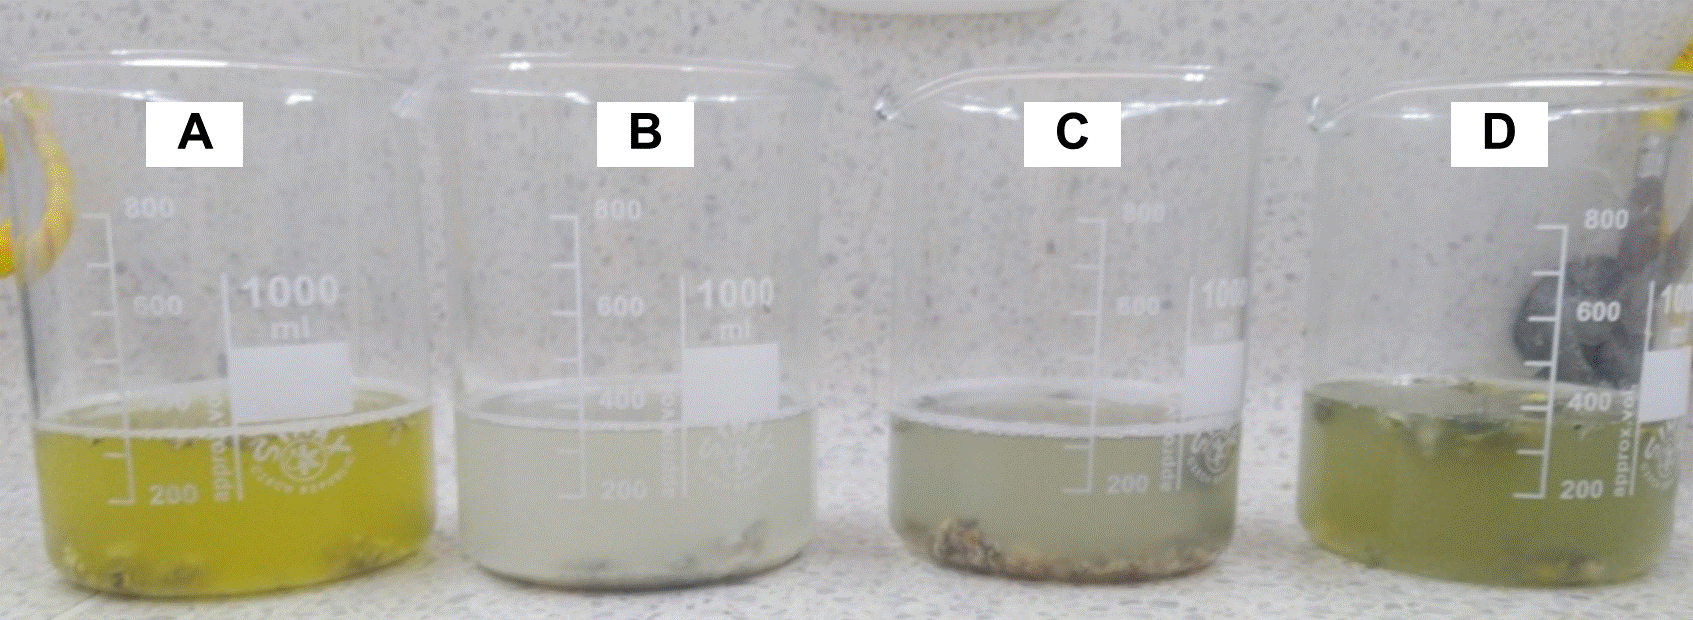
\includegraphics[width=3.55208in,height=\textheight,keepaspectratio]{images/3_DCA/sustrato.png}

}

\caption{Nota: Dilución de conidios y sustrato, en solución tween80®
0,01\%: Avena (A); Arroz (B); Cebada (C); Maíz Partido (D).}

\end{figure}%

\hfill\break
La evaluación in vitro reveló que las concentraciones de extracto crudo
de 4,0 al 6,0\% generaron Porcentajes de Inhibición del Crecimiento
micelial (PICM) del 40 al 50 \% respectivamente al quinto día después de
la inoculación (ddi) \textbf{(Figura 2)}.

\textbf{Figura 2.\\
}Efecto de los tratamientos in vitro frente al crecmiento de
\emph{Colletotrichum musae.}

\begin{figure}[H]

{\centering \pandocbounded{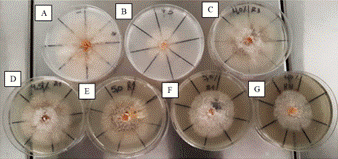
\includegraphics[keepaspectratio]{images/3_DCA/experimentoinvitro.png}}

}

\caption{Nota: Prueba de inhibición in vitro de Colletotrichum musae,
frente a diferentes tratamientos. (A) Testigo negativo; (B) Testigo
positivo (Amistar a 60mg/100mL); (C) Extracto de \emph{Penicillium} sp.,
al 4\%; (D) Extracto de \emph{Penicillium} sp., al 4,5\%; (E) Extracto
de \emph{Penicillium} sp., al 5\%; (F) Extracto de \emph{Penicillium}
sp., al 5,5\%; (G) Extracto de \emph{Penicillium} sp., al 6\%.}

\end{figure}%

\hfill\break
Por otro lado,~ los ensayos in vivo evidenciaron una mayor eficacia del
extracto crudo, donde las concentraciones de 8, 9, 10, 11, 12 y 13\%
generaron porcentajes de inhibición del área de la lesión (PIAL) de 60,
55, 70, 72, 77 y 80\% respectivamente \textbf{(Figura 3)}, sugiriendo
que Penicillium digitatum podría representar una alternativa viable para
el manejo preventivo de la antracnosis del banano.

\textbf{Figura 3.}\\
Efecto in vivo de bananos infectados con \emph{Colletotrichum musae} en
los tratamientos.

\begin{figure}[H]

{\centering \pandocbounded{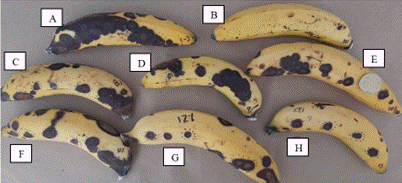
\includegraphics[keepaspectratio]{images/3_DCA/experimentobananos.png}}

}

\caption{Nota: Experimento in vivo de los bananos infectados con 107
conidios de Colletotrichum musae, frente a tratamientos (A los 7 días de
la inoculación). (A) Testigo negativo; (B) Azoxystrobin (Testigo
positivo); Extractos de Penicillium sp. a (C) 8\%; (D) 9\%; (E) 10\%;
(F) 11\%; (G) 12\%; (H) 13\%.}

\end{figure}%

\textbf{\hfill\break
Para mayor información puede consultar:} Mejía-Sarmiento, J. S. (2022).
Evaluación de Extracto Crudo de Penicillium sp. para la Inhibición del
Crecimiento in vitro e in vivo de Colletotrichum musae (Berk. y M. A.
Curtis) Arx. Agente Causal de Antracnosis en Banano {[}Tesis de
pregrado, Universidad de Santander UDES{]}. Repositorio Institucional
UDES. \url{https://repositorio.udes.edu.co/handle/001/8674}

\subsection{Estructura de la base de
datos}\label{estructura-de-la-base-de-datos}

La base de datos utilizada en este análisis corresponde a los resultados
de un experimento agrícola que evalúa el comportamiento de cuatro
cultivos diferentes bajo condiciones similares de manejo. La tabla
contiene tres columnas principales:

\begin{longtable}[]{@{}
  >{\raggedright\arraybackslash}p{(\linewidth - 2\tabcolsep) * \real{0.2778}}
  >{\raggedright\arraybackslash}p{(\linewidth - 2\tabcolsep) * \real{0.7222}}@{}}
\toprule\noalign{}
\begin{minipage}[b]{\linewidth}\raggedright
Variable
\end{minipage} & \begin{minipage}[b]{\linewidth}\raggedright
Descripción
\end{minipage} \\
\midrule\noalign{}
\endhead
\bottomrule\noalign{}
\endlastfoot
\texttt{Tratamiento} & Tipo de cultivo evaluado. Incluye cuatro niveles:
Arroz, Avena, Cebada y Maíz. \\
\texttt{Repetición} & Número de repetición del tratamiento (del 1 al 4).
Permite el análisis estadístico con replicación. \\
\texttt{Resultado} & Valor numérico correspondiente a la variable
respuesta medida (por ejemplo, rendimiento en kg/ha). \\
\end{longtable}

\textbf{Pasos para trabajar con R o RStudio:}

Especificar el directorio que me interesa donde se encuentra la base de
datos.

\begin{tcolorbox}[enhanced jigsaw, titlerule=0mm, arc=.35mm, rightrule=.15mm, bottomrule=.15mm, leftrule=.75mm, colbacktitle=quarto-callout-tip-color!10!white, colframe=quarto-callout-tip-color-frame, coltitle=black, opacityback=0, colback=white, toptitle=1mm, opacitybacktitle=0.6, toprule=.15mm, bottomtitle=1mm, title=\textcolor{quarto-callout-tip-color}{\faLightbulb}\hspace{0.5em}{Antes e inciar}, left=2mm, breakable]

R lee / (slash o division) y no el de Windows \textbackslash{}

En \textbf{R}, \texttt{setwd()} es una función que significa
\textbf{``set working directory''} o ``establecer el directorio de
trabajo''. Se utiliza para \textbf{definir la carpeta predeterminada} en
la que R buscará archivos para leer y donde guardará archivos por
defecto.\\

Por ejemplo: setwd (``D:/OneDrive - Universidad de Santander/Material
Docente 2025/CodigoR''\,``)

\end{tcolorbox}

\textbf{Lectura de datos}

\begin{Shaded}
\begin{Highlighting}[]
\FunctionTok{library}\NormalTok{(readxl)}
\end{Highlighting}
\end{Shaded}

\begin{verbatim}
Warning: package 'readxl' was built under R version 4.3.3
\end{verbatim}

\begin{Shaded}
\begin{Highlighting}[]
\NormalTok{DCA }\OtherTok{\textless{}{-}} \FunctionTok{read\_excel}\NormalTok{(}\StringTok{"C:/R{-}Proyectos/r{-}para{-}mi/data/dca.xlsx"}\NormalTok{)}

\FunctionTok{View}\NormalTok{(DCA)}
\FunctionTok{attach}\NormalTok{(DCA)}
\FunctionTok{names}\NormalTok{(DCA)}
\end{Highlighting}
\end{Shaded}

\begin{verbatim}
[1] "Tratamiento" "Repeticion"  "Resultado"  
\end{verbatim}

\begin{Shaded}
\begin{Highlighting}[]
\FunctionTok{str}\NormalTok{(DCA)}
\end{Highlighting}
\end{Shaded}

\begin{verbatim}
tibble [16 x 3] (S3: tbl_df/tbl/data.frame)
 $ Tratamiento: chr [1:16] "Arroz" "Arroz" "Arroz" "Arroz" ...
 $ Repeticion : num [1:16] 1 2 3 4 1 2 3 4 1 2 ...
 $ Resultado  : num [1:16] 8.76 8.74 8.72 8.72 8.39 ...
\end{verbatim}

\begin{Shaded}
\begin{Highlighting}[]
\FunctionTok{summary}\NormalTok{(DCA}\SpecialCharTok{$}\NormalTok{Resultado)}
\end{Highlighting}
\end{Shaded}

\begin{verbatim}
   Min. 1st Qu.  Median    Mean 3rd Qu.    Max. 
  8.341   8.635   8.792   8.775   8.954   9.141 
\end{verbatim}

\textbf{Análisis de la Varianza - ANOVA}

Cuando se desea saber si varios grupos (Ej. tratamientos) presentan
diferencias reales en sus promedios, una de las herramientas
estadísticas más utilizadas es el Análisis de la Varianza, conocido como
ANOVA. Esta técnica permite examinar si los valores medios de tres o más
grupos son lo suficientemente distintos como para concluir que no se
trata de simples fluctuaciones aleatorias.

El enfoque de ANOVA se basa en comparar dos tipos de variación: por un
lado, l\textbf{a variabilidad que se observa entre los distintos
grupos}, y por otro, \textbf{la variabilidad que existe dentro de cada
grupo individual}.

Si al analizar los datos se encuentra que la variación entre los grupos
supera notablemente la que ocurre dentro de ellos, es razonable pensar
que las diferencias en los promedios reflejan algo más que el azar. En
cambio, si la variabilidad interna es más pronunciada, entonces es
posible que las diferencias observadas no sean significativas y
respondan a variaciones normales del comportamiento de los datos.

\textbf{Código de R para ANOVA}

\begin{Shaded}
\begin{Highlighting}[]
\NormalTok{Anova}\OtherTok{\textless{}{-}}\FunctionTok{aov}\NormalTok{(Resultado}\SpecialCharTok{\textasciitilde{}}\NormalTok{Tratamiento, }\AttributeTok{data=}\NormalTok{DCA)}
\FunctionTok{summary}\NormalTok{(Anova)}
\end{Highlighting}
\end{Shaded}

\begin{verbatim}
            Df Sum Sq Mean Sq F value   Pr(>F)    
Tratamiento  3 1.1794  0.3931   660.4 1.39e-13 ***
Residuals   12 0.0071  0.0006                     
---
Signif. codes:  0 '***' 0.001 '**' 0.01 '*' 0.05 '.' 0.1 ' ' 1
\end{verbatim}

\textbf{Interpretación:} La prueba ANOVA muestra diferencias
significativas entre los tratamientos (p \textless{} 0.001). El valor de
F (660.4) indica que la variación entre tratamientos es mucho mayor que
la variación dentro de los grupos, lo que sugiere que al menos uno de
los tratamientos afecta significativamente el resultado.

\textbf{Modelo Lineal}

\begin{Shaded}
\begin{Highlighting}[]
\NormalTok{modelo}\OtherTok{=}\FunctionTok{lm}\NormalTok{(Resultado}\SpecialCharTok{\textasciitilde{}}\NormalTok{(Tratamiento))}
\FunctionTok{summary}\NormalTok{(modelo)}
\end{Highlighting}
\end{Shaded}

\begin{verbatim}

Call:
lm(formula = Resultado ~ (Tratamiento))

Residuals:
      Min        1Q    Median        3Q       Max 
-0.038397 -0.016205  0.001983  0.012013  0.040116 

Coefficients:
                  Estimate Std. Error t value Pr(>|t|)    
(Intercept)        8.73389    0.01220 715.921  < 2e-16 ***
TratamientoAvena  -0.35848    0.01725 -20.778 8.93e-11 ***
TratamientoCebada  0.12669    0.01725   7.343 8.94e-06 ***
TratamientoMaiz    0.39630    0.01725  22.970 2.75e-11 ***
---
Signif. codes:  0 '***' 0.001 '**' 0.01 '*' 0.05 '.' 0.1 ' ' 1

Residual standard error: 0.0244 on 12 degrees of freedom
Multiple R-squared:  0.994, Adjusted R-squared:  0.9925 
F-statistic: 660.4 on 3 and 12 DF,  p-value: 1.393e-13
\end{verbatim}

\textbf{Interpretación:} El modelo lineal confirma que el tratamiento
influye significativamente en los resultados (p \textless{} 0.001). El
tratamiento ``Arroz'' actúa como referencia, con una media estimada de
8.73. Comparado con este:

\begin{verbatim}
Avena presenta una media significativamente menor (–0.36, p < 0.001).

Cebada muestra un aumento moderado (+0.13, p < 0.001).

Maíz tiene el mayor incremento (+0.40, p < 0.001).
\end{verbatim}

El modelo explica el 99.4\% de la variabilidad en los datos (R² =
0.994), y el error estándar residual es bajo (0.0244), lo que indica un
ajuste excelente.

\textbf{Gráfico Boxplot}

Se toma el Tratamiento para hacer un boxplot utilizando la variable
``Resultado'', pero primero se transformar en factor la variable
Tratamiento:

\begin{Shaded}
\begin{Highlighting}[]
\FunctionTok{library}\NormalTok{(ggplot2)}

\NormalTok{DCA}\SpecialCharTok{$}\NormalTok{Treatamiento}\OtherTok{\textless{}{-}}\FunctionTok{factor}\NormalTok{(DCA}\SpecialCharTok{$}\NormalTok{Tratamiento) }\CommentTok{\#transformamos una variable númerica en un factor categórico}
\FunctionTok{ggplot}\NormalTok{(DCA, }\FunctionTok{aes}\NormalTok{(}\AttributeTok{x =}\NormalTok{ Tratamiento, }\AttributeTok{y =}\NormalTok{ Resultado, }\AttributeTok{fill=}\NormalTok{Tratamiento)) }\SpecialCharTok{+} 
  \FunctionTok{geom\_boxplot}\NormalTok{()}
\end{Highlighting}
\end{Shaded}

\pandocbounded{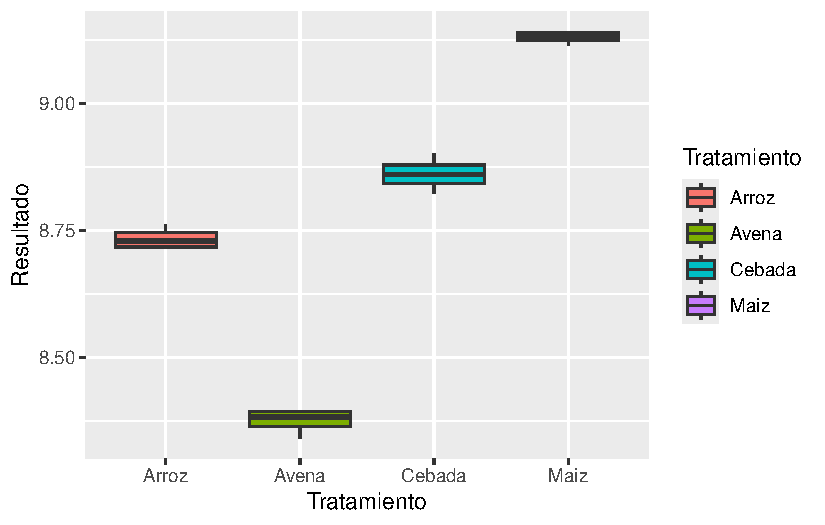
\includegraphics[keepaspectratio]{Chapter_02_files/figure-pdf/unnamed-chunk-4-1.pdf}}

\textbf{Interpretación:} Las diferencias en las medianas entre
tratamientos son claras y consistentes con los resultados del ANOVA y
del modelo lineal, lo que sugiere un efecto significativo del tipo de
cultivo sobre la variable resultado.

\textbf{Supuestos del diseño}

\textbf{Normalidad:} Para verificar la normalidad de los residuos
utilizaremos la prueba de Shapiro-Wilks cuyo script es el siguiente:

\begin{Shaded}
\begin{Highlighting}[]
\FunctionTok{shapiro.test}\NormalTok{(}\FunctionTok{residuals}\NormalTok{(Anova))}
\end{Highlighting}
\end{Shaded}

\begin{verbatim}

    Shapiro-Wilk normality test

data:  residuals(Anova)
W = 0.97944, p-value = 0.959
\end{verbatim}

\textbf{Interpretación:} El test de Shapiro-Wilk aplicado a los residuos
del modelo ANOVA devuelve un valor de p = 0.959, que es mucho mayor que
0.05. Esto indica que no hay evidencia estadística para rechazar la
hipótesis nula de normalidad. Por lo tanto, se concluye que los residuos
del modelo siguen una distribución normal, cumpliendo así uno de los
supuestos fundamentales del análisis de varianza.

\textbf{Gráficos para evaluar la normalidad}

Para construir el gráfico QQ (QQ plot) y evaluar la normalidad de los
datos, se utiliza la función correspondiente del paquete car. Si no está
instalado previamente, es necesario instalar también el paquete auxiliar
carData.

Instalación (si es necesario) install.packages (``car'')
install.packages (``carData'') install.packages (``dplyr'')
install.packages (``purrr'')

\textbf{Cargar los paquetes (librerias)}

\begin{Shaded}
\begin{Highlighting}[]
\FunctionTok{library}\NormalTok{(car) }\CommentTok{\#Grafico de QQ plot}
\FunctionTok{library}\NormalTok{(carData)}
\FunctionTok{library}\NormalTok{(dplyr)}
\FunctionTok{library}\NormalTok{(purrr)}

\FunctionTok{qqPlot}\NormalTok{(Anova)}
\end{Highlighting}
\end{Shaded}

\pandocbounded{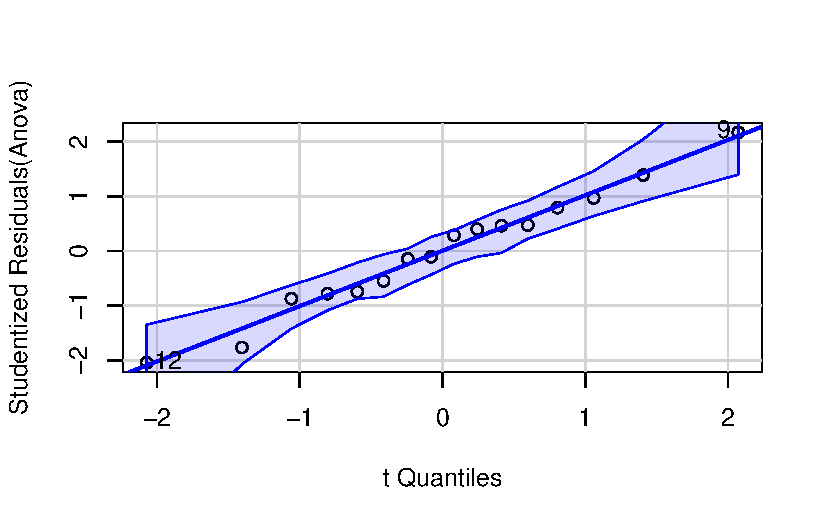
\includegraphics[keepaspectratio]{Chapter_02_files/figure-pdf/unnamed-chunk-6-1.pdf}}

\begin{verbatim}
[1]  9 12
\end{verbatim}

\textbf{Interpretación:} El gráfico QQ muestra que los residuos
estandarizados del modelo ANOVA se alinean adecuadamente con la línea
diagonal, lo que indica que su distribución es aproximadamente normal.
La mayoría de los puntos se ubican dentro de la banda de confianza, y no
se observan desviaciones sistemáticas. Esta gráfica complementa el
resultado del test de Shapiro-Wilk (p = 0.959), confirmando que se
cumple el supuesto de normalidad de los residuos en el modelo.

\textbf{Homocedasticidad:} Para evaluar el supuesto de homogeneidad de
varianzas entre los grupos (homocedasticidad), se aplicará la prueba de
Bartlett, la cual es apropiada cuando los datos provienen de poblaciones
aproximadamente normales. Esta prueba contrasta la hipótesis nula de
igualdad de varianzas frente a la alternativa de varianzas diferentes.
El procedimiento se implementa mediante el siguiente script:

\begin{Shaded}
\begin{Highlighting}[]
\FunctionTok{bartlett.test}\NormalTok{(Resultado}\SpecialCharTok{\textasciitilde{}}\NormalTok{Tratamiento, }\AttributeTok{data=}\NormalTok{DCA)}
\end{Highlighting}
\end{Shaded}

\begin{verbatim}

    Bartlett test of homogeneity of variances

data:  Resultado by Tratamiento
Bartlett's K-squared = 2.2722, df = 3, p-value = 0.5179
\end{verbatim}

\textbf{Interpretación:} Dado que el valor de p es mayor que 0.05 (p =
0.5179), no se rechaza la hipótesis nula. Por tanto, se asume que las
varianzas entre los tratamientos son homogéneas, cumpliéndose este
supuesto clave para el análisis de varianza y para la aplicación de
pruebas a posteriori como LSD.

\textbf{Pruebas aposteriori} Para identificar diferencias específicas
entre las medias de los tratamientos, una vez detectada significancia en
el análisis de varianza, se aplicará una prueba de comparaciones
múltiples a posteriori. En este caso, se empleará la técnica LSD (Least
Significant Difference), que permite realizar comparaciones pareadas
entre tratamientos asumiendo homogeneidad de varianzas.

La implementación de esta prueba requiere la carga del paquete
agricolae, utilizando el siguiente script. Instalación si es necesario:
install.packages(``agricolae''). Carga del paquete: library(agricolae).

\begin{Shaded}
\begin{Highlighting}[]
\FunctionTok{library}\NormalTok{(agricolae)}
\NormalTok{Grupos }\OtherTok{\textless{}{-}} \FunctionTok{LSD.test}\NormalTok{(}\AttributeTok{y =}\NormalTok{ Anova, }\AttributeTok{trt =} \StringTok{"Tratamiento"}\NormalTok{, }\AttributeTok{group =}\NormalTok{ T, }\AttributeTok{console =}\NormalTok{ T)}
\end{Highlighting}
\end{Shaded}

\begin{verbatim}

Study: Anova ~ "Tratamiento"

LSD t Test for Resultado 

Mean Square Error:  0.0005953124 

Tratamiento,  means and individual ( 95 %) CI

       Resultado        std r         se      LCL      UCL      Min      Max
Arroz   8.733890 0.02192214 4 0.01219951 8.707310 8.760471 8.715318 8.762183
Avena   8.375414 0.02519485 4 0.01219951 8.348834 8.401995 8.341039 8.395990
Cebada  8.860578 0.03330518 4 0.01219951 8.833998 8.887159 8.822181 8.900695
Maiz    9.130190 0.01251613 4 0.01219951 9.103609 9.156770 9.113429 9.140539
            Q25      Q50      Q75
Arroz  8.717232 8.729030 8.745688
Avena  8.364419 8.382314 8.393309
Cebada 8.842075 8.859719 8.878222
Maiz   9.124249 9.133395 9.139335

Alpha: 0.05 ; DF Error: 12
Critical Value of t: 2.178813 

least Significant Difference: 0.03759044 

Treatments with the same letter are not significantly different.

       Resultado groups
Maiz    9.130190      a
Cebada  8.860578      b
Arroz   8.733890      c
Avena   8.375414      d
\end{verbatim}

\textbf{Intrepretación:} La prueba LSD reveló que los cuatro
tratamientos presentan diferencias estadísticamente significativas entre
sus medias. El tratamiento Maíz obtuvo el mayor rendimiento promedio,
seguido por Cebada, Arroz y Avena, en ese orden descendente.

Otra opcion cuando cambiamos el argumento ``group'' a F(false), se
interpreta a mi parecer de forma mas sencilla la diferencia entre las
medias.A continuación, se presentan las pruebas de comparaciones
múltiples a posteriori aplicadas al modelo de ANOVA ajustado. Se
incluyen la prueba LSD, la prueba de Tukey y el test de Scheffé, las
cuales permiten identificar diferencias estadísticamente significativas
entre los tratamientos evaluados:

\begin{Shaded}
\begin{Highlighting}[]
\NormalTok{Grupos}\OtherTok{\textless{}{-}} \FunctionTok{LSD.test}\NormalTok{(}\AttributeTok{y =}\NormalTok{ Anova, }\AttributeTok{trt =} \StringTok{"Tratamiento"}\NormalTok{, }\AttributeTok{group =}\NormalTok{ F, }\AttributeTok{console =}\NormalTok{ T)}
\end{Highlighting}
\end{Shaded}

\begin{verbatim}

Study: Anova ~ "Tratamiento"

LSD t Test for Resultado 

Mean Square Error:  0.0005953124 

Tratamiento,  means and individual ( 95 %) CI

       Resultado        std r         se      LCL      UCL      Min      Max
Arroz   8.733890 0.02192214 4 0.01219951 8.707310 8.760471 8.715318 8.762183
Avena   8.375414 0.02519485 4 0.01219951 8.348834 8.401995 8.341039 8.395990
Cebada  8.860578 0.03330518 4 0.01219951 8.833998 8.887159 8.822181 8.900695
Maiz    9.130190 0.01251613 4 0.01219951 9.103609 9.156770 9.113429 9.140539
            Q25      Q50      Q75
Arroz  8.717232 8.729030 8.745688
Avena  8.364419 8.382314 8.393309
Cebada 8.842075 8.859719 8.878222
Maiz   9.124249 9.133395 9.139335

Alpha: 0.05 ; DF Error: 12
Critical Value of t: 2.178813 

Comparison between treatments means

               difference pvalue signif.        LCL         UCL
Arroz - Avena   0.3584760      0     ***  0.3208855  0.39606642
Arroz - Cebada -0.1266884      0     *** -0.1642788 -0.08909794
Arroz - Maiz   -0.3962994      0     *** -0.4338899 -0.35870901
Avena - Cebada -0.4851644      0     *** -0.5227548 -0.44757392
Avena - Maiz   -0.7547754      0     *** -0.7923659 -0.71718499
Cebada - Maiz  -0.2696111      0     *** -0.3072015 -0.23202064
\end{verbatim}

\textbf{Interpretación:} todas las diferencias entre tratamientos son
altamente significativas (p \textless{} 0.001). Esto confirma que
ninguno de los tratamientos comparte una media similar.

\begin{Shaded}
\begin{Highlighting}[]
\FunctionTok{TukeyHSD}\NormalTok{(Anova) }
\end{Highlighting}
\end{Shaded}

\begin{verbatim}
  Tukey multiple comparisons of means
    95% family-wise confidence level

Fit: aov(formula = Resultado ~ Tratamiento, data = DCA)

$Tratamiento
                   diff         lwr        upr   p adj
Avena-Arroz  -0.3584760 -0.40969759 -0.3072544 0.0e+00
Cebada-Arroz  0.1266884  0.07546677  0.1779100 4.6e-05
Maiz-Arroz    0.3962994  0.34507784  0.4475211 0.0e+00
Cebada-Avena  0.4851644  0.43394275  0.5363860 0.0e+00
Maiz-Avena    0.7547754  0.70355383  0.8059970 0.0e+00
Maiz-Cebada   0.2696111  0.21838947  0.3208327 0.0e+00
\end{verbatim}

\textbf{Interpretación:} La prueba de Tukey también confirma diferencias
estadísticamente significativas en todas las comparaciones, manteniendo
control del error familiar. El gráfico generado muestra intervalos de
confianza del 95\% que no se solapan, lo que respalda visualmente los
resultados.

\begin{Shaded}
\begin{Highlighting}[]
\FunctionTok{plot}\NormalTok{(}\FunctionTok{TukeyHSD}\NormalTok{(Anova))}
\end{Highlighting}
\end{Shaded}

\pandocbounded{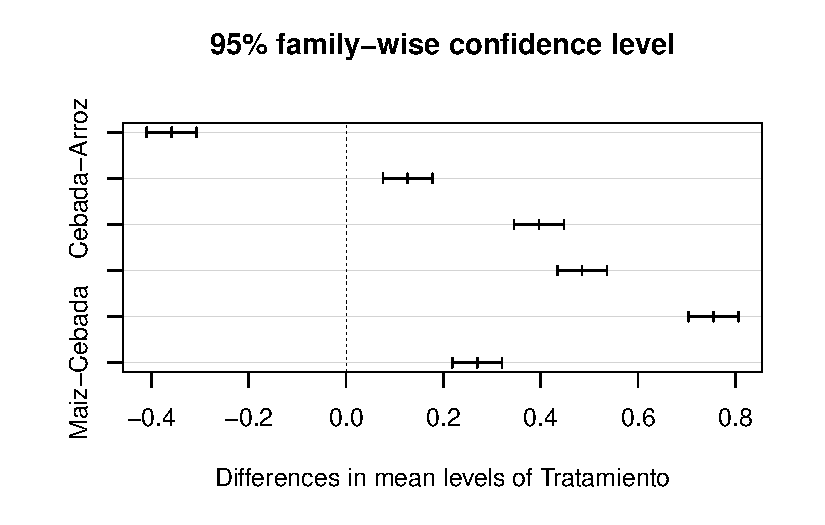
\includegraphics[keepaspectratio]{Chapter_02_files/figure-pdf/unnamed-chunk-11-1.pdf}}

\textbf{Interpretación:} El gráfico muestra los intervalos de confianza
del 95\,\% para las diferencias de medias entre los tratamientos,
ajustados por comparaciones múltiples (family-wise). Ninguno de los
intervalos cruza la línea vertical en cero, lo cual indica que todas las
comparaciones entre pares de tratamientos son estadísticamente
significativas. La diferencia más grande se observa entre Maíz y Avena,
mientras que la más pequeña, aunque significativa, es entre Cebada y
Arroz. Este resultado es coherente con los análisis previos (ANOVA, LSD
y Scheffé), y respalda que cada tratamiento tiene un efecto
significativamente distinto sobre la variable ``Resultado''.

\begin{Shaded}
\begin{Highlighting}[]
\FunctionTok{scheffe.test}\NormalTok{(Anova, }\StringTok{"Tratamiento"}\NormalTok{,}\AttributeTok{console=}\ConstantTok{TRUE}\NormalTok{)}
\end{Highlighting}
\end{Shaded}

\begin{verbatim}

Study: Anova ~ "Tratamiento"

Scheffe Test for Resultado 

Mean Square Error  : 0.0005953124 

Tratamiento,  means

       Resultado        std r         se      Min      Max      Q25      Q50
Arroz   8.733890 0.02192214 4 0.01219951 8.715318 8.762183 8.717232 8.729030
Avena   8.375414 0.02519485 4 0.01219951 8.341039 8.395990 8.364419 8.382314
Cebada  8.860578 0.03330518 4 0.01219951 8.822181 8.900695 8.842075 8.859719
Maiz    9.130190 0.01251613 4 0.01219951 9.113429 9.140539 9.124249 9.133395
            Q75
Arroz  8.745688
Avena  8.393309
Cebada 8.878222
Maiz   9.139335

Alpha: 0.05 ; DF Error: 12 
Critical Value of F: 3.490295 

Minimum Significant Difference: 0.05582762 

Means with the same letter are not significantly different.

       Resultado groups
Maiz    9.130190      a
Cebada  8.860578      b
Arroz   8.733890      c
Avena   8.375414      d
\end{verbatim}

\textbf{Interpretación:} A pesar de ser una prueba más conservadora, el
test de Scheffé también encontró diferencias significativas entre todos
los tratamientos. El análisis agrupó los tratamientos en distintos
niveles.Mínima diferencia significativa (Scheffé): 0.0558. Valor crítico
de F: 3.4903

\textbf{Conclusión general} Las tres pruebas aplicadas (LSD, Tukey y
Scheffé) coinciden en que todos los tratamientos difieren
significativamente entre sí. El tratamiento con mayor rendimiento fue
Maíz, seguido por Cebada, Arroz y Avena, en orden descendente. Esto
respalda la conclusión de que el tipo de tratamiento influye de manera
significativa sobre la variable respuesta.

\subsubsection{2.2.2 Diseño de bloques completamente al azar
OK}\label{diseuxf1o-de-bloques-completamente-al-azar-ok}

\subsubsection{2.2.3 Diseño longitudinal (ANOVA de medidas repetidas)
OK}\label{diseuxf1o-longitudinal-anova-de-medidas-repetidas-ok}

\subsection{Problema}\label{problema-1}

\begin{tcolorbox}[enhanced jigsaw, titlerule=0mm, arc=.35mm, rightrule=.15mm, bottomrule=.15mm, leftrule=.75mm, colbacktitle=quarto-callout-important-color!10!white, colframe=quarto-callout-important-color-frame, coltitle=black, opacityback=0, colback=white, toptitle=1mm, opacitybacktitle=0.6, toprule=.15mm, bottomtitle=1mm, title=\textcolor{quarto-callout-important-color}{\faExclamation}\hspace{0.5em}{Importante}, left=2mm, breakable]

\textbf{Metodología:} Se realizó un diseño de medidas repetidas en el
tiempo, donde la variable independiente fue cada una de las
concentraciones del extracto y los testigos; y la variable respuesta
fueron: Porcentaje de Inhibición del Área de la Lesió (PIAL) y
Porcentaje de Inhibición del Crecimiento Micelial (PICM).

\end{tcolorbox}

\bookmarksetup{startatroot}

\chapter{Parte III: Uso de Inteligencia Artificial para la simulación de
datos}\label{parte-iii-uso-de-inteligencia-artificial-para-la-simulaciuxf3n-de-datos}

\section{Uso de Inteligencia Artificial para la simulación de
datos.}\label{uso-de-inteligencia-artificial-para-la-simulaciuxf3n-de-datos.}

\subsection{}\label{section}

\bookmarksetup{startatroot}

\chapter*{Referencias}\label{referencias}
\addcontentsline{toc}{chapter}{Referencias}

\markboth{Referencias}{Referencias}

\phantomsection\label{refs}
\begin{CSLReferences}{1}{0}
\bibitem[\citeproctext]{ref-Aria2017}
Aria, M., \& Cuccurullo, C. (2017). {bibliometrix: An R-tool for
comprehensive science mapping analysis}. \emph{Journal of Informetrics},
\emph{11}(4), 959-975. \url{https://doi.org/10.1016/j.joi.2017.08.007}

\bibitem[\citeproctext]{ref-Arias2007}
Arias B., C. L. (2007). Control Qu{í}mico de la Antracnosis del Mango
({Mangifera indica L.}) en pre y postcosecha. \emph{Bioagro},
\emph{19}(1), 19-25.
\url{http://www.ucla.edu.ve/bioagro/Rev19(1)/3.\%20Control\%20qu\%C3\%ADmico\%20de\%20la\%20antracnosis.pdf}

\bibitem[\citeproctext]{ref-Auguie2017}
Auguie, B. (2017). \emph{{gridExtra: Miscellaneous Functions for "Grid"
Graphics}}. \url{https://CRAN.R-project.org/package=gridExtra}

\bibitem[\citeproctext]{ref-Chang2021}
Chang, W., Cheng, J., Allaire, J., Xie, Y., \& McPherson, J. (2021).
\emph{shiny: Web Application Framework for R}.
\url{https://CRAN.R-project.org/package=shiny}

\bibitem[\citeproctext]{ref-Fox2019}
Fox, J., \& Weisberg, S. (2019). \emph{{An R Companion to Applied
Regression}} (3.ª ed.). Sage Publications.
\url{https://uk.sagepub.com/en-gb/eur/an-r-companion-to-applied-regression/book246125}

\bibitem[\citeproctext]{ref-gutierrez2012analisis}
Gutiérrez Pulido, H., \& Vara Salazar, R. de la. (2012).
\emph{An{á}lisis y dise{ñ}o de experimentos} (3.ª ed.).
McGraw-Hill/Interamericana Editores, S.A. de C.V.

\bibitem[\citeproctext]{ref-Lahti2017}
Lahti, L., \& Shetty, S. (2017). \emph{{microbiome R package}}.
\url{http://microbiome.github.io/microbiome}

\bibitem[\citeproctext]{ref-Love2014}
Love, M. I., Huber, W., \& Anders, S. (2014). {Moderated estimation of
fold change and dispersion for RNA-seq data with DESeq2}. \emph{Genome
Biology}, \emph{15}(12), 550.
\url{https://doi.org/10.1186/s13059-014-0550-8}

\bibitem[\citeproctext]{ref-McMurdie2013}
McMurdie, P. J., \& Holmes, S. (2013). {phyloseq: An R package for
reproducible interactive analysis and graphics of microbiome census
data}. \emph{PLOS ONE}, \emph{8}(4), e61217.
\url{https://doi.org/10.1371/journal.pone.0061217}

\bibitem[\citeproctext]{ref-Mendiburu2020}
Mendiburu, F. (2020). \emph{agricolae: Statistical Procedures for
Agricultural Research}.
\url{https://CRAN.R-project.org/package=agricolae}

\bibitem[\citeproctext]{ref-Mohammadi2019}
Mohammadi, R., Ghomi, S. M. T. F., \& Nazari, F. (2019). {The
application of R software for the assessment of microbial fermentation
processes}. \emph{Journal of Microbiological Methods}, \emph{156},
54-58. \url{https://doi.org/10.1016/j.mimet.2018.12.003}

\bibitem[\citeproctext]{ref-Navarro2015}
Navarro, D. J. (2015). \emph{{Learning Statistics with R: A tutorial for
psychology students and other beginners}} (Versión 0.5). University of
Adelaide. \url{https://learningstatisticswithr.com/}

\bibitem[\citeproctext]{ref-Oksanen2020}
Oksanen, J., Blanchet, F. G., Friendly, M., Kindt, R., Legendre, P.,
McGlinn, D., Minchin, P. R., O'Hara, R. B., Simpson, G. L., Solymos, P.,
Stevens, M. H. H., Szoecs, E., \& Wagner, H. (2020). \emph{{vegan:
Community ecology package}}.
\url{https://CRAN.R-project.org/package=vegan}

\bibitem[\citeproctext]{ref-Pinheiro2025}
Pinheiro, J., Bates, D., DebRoy, S., Sarkar, D., \& Team, R. C. (2025).
\emph{{nlme: Linear and nonlinear mixed effects models}}.
\url{https://CRAN.R-project.org/package=nlme}

\bibitem[\citeproctext]{ref-Rcore2021}
R Core Team. (2021). \emph{R: A Language and Environment for Statistical
Computing}. R Foundation for Statistical Computing.
\url{https://www.R-project.org/}

\bibitem[\citeproctext]{ref-Ritz2005}
Ritz, C., \& Streibig, J. C. (2005). {Bioassay analysis using R}.
\emph{Journal of Statistical Software}, \emph{12}(5), 1-22.
\url{https://doi.org/10.18637/jss.v012.i05}

\bibitem[\citeproctext]{ref-Rohart2017}
Rohart, F., Gautier, B., Singh, A., \& Lê Cao, K.-A. (2017). {mixOmics:
An R package for 'omics feature selection and multiple data
integration}. \emph{PLOS Computational Biology}, \emph{13}(11),
e1005752. \url{https://doi.org/10.1371/journal.pcbi.1005752}

\bibitem[\citeproctext]{ref-Vasquez-Castillo2019}
Vásquez-Castillo, W., Racines-Oliva, M., Moncayo, P., Viera, W., \&
Seraquive, M. (2019). Calidad del fruto y p{é}rdidas postcosecha de
banano org{á}nico ({Musa acuminata}) en el {Ecuador}. \emph{Enfoque
UTE}, \emph{10}(4), 57-66.
\url{https://doi.org/10.29019/enfoque.v10n4.545}

\bibitem[\citeproctext]{ref-Wickham2016}
Wickham, H. (2016). \emph{{ggplot2: Elegant graphics for data analysis}}
(2.ª ed.). Springer. \url{https://doi.org/10.1007/978-3-319-24277-4}

\bibitem[\citeproctext]{ref-Wickham2019}
Wickham, H., Averick, M., Bryan, J., Chang, W., McGowan, L. D.,
François, R., Grolemund, G., Hayes, A., Henry, L., Hester, J., Kuhn, M.,
Pedersen, T. L., Miller, E., Bache, S. M., Müller, K., Ooms, J.,
Robinson, D., Seidel, D. P., Spinu, V., \& Yutani, H. (2019). {Welcome
to the tidyverse}. \emph{Journal of Open Source Software}, \emph{4}(43),
1686. \url{https://doi.org/10.21105/joss.01686}

\bibitem[\citeproctext]{ref-wickham2015}
Wickham, H., \& Bryan, J. (2015). \emph{readxl: Read Excel Files}.
\url{https://CRAN.R-project.org/package=readxl}

\bibitem[\citeproctext]{ref-Wickham2017r4ds}
Wickham, H., \& Grolemund, G. (2017). \emph{R for Data Science: Import,
Tidy, Transform, Visualize, and Model Data}. O'Reilly Media.
\url{https://r4ds.had.co.nz}

\bibitem[\citeproctext]{ref-Yu2017}
Yu, G., Smith, D. K., Zhu, H., Guan, Y., \& Lam, T. T. Y. (2017).
{ggtree: An R package for visualization and annotation of phylogenetic
trees with their covariates and other associated data}. \emph{Methods in
Ecology and Evolution}, \emph{8}(1), 28-36.
\url{https://doi.org/10.1111/2041-210X.12628}

\bibitem[\citeproctext]{ref-Zhou2012}
Zhou, B., Xiao, J. F., Tuli, L., \& Ressom, H. W. (2012). LC-MS-based
metabolomics. \emph{Molecular BioSystems}, \emph{8}(2), 470-481.
\url{https://doi.org/10.1039/c1mb05350g}

\end{CSLReferences}




\end{document}
